\chapter{Поисковые методы идентификации}

\section{Основные понятия и параметры поисковых систем идентификации}  % {{{1

\subsection{Априорная и текущая информация}  % {{{2

Без априорной информации невозможно построение
работоспособной системы идентификации. Основные
априорные величины определяются на этапе постановки
задачи идентификации. В первую очередь это
параметры масштаба: множество допустимых
значений параметров \label{atu:d:p_set}\( \mathcal{P}\),
характерное время работы
идентифицируемой системы~$T$, а также
требуемая точность и скорость идентификации
(могут быть заданы различными способами).
В этот список может входить и ограничения на динамику изменения параметра.
В процессе работы эти параметры могут уточнятся по текущей информации.

Следующую часть априорной (по отношению к идентификации) информации
предоставляет процесс синтеза критерия идентификации.
В первую очередь, это сам вид критерия. Им определятся
как диапазон изменения величины этого критерия $\Delta q$, так и
динамические свойства:
зависимости $\sigma_q(\tau_q)$ или  $\sigma_q(a_q)$,
в простейших случаях, при заданной точности --- характерное/минимально время
оценивания \(\tau_{q,\min}\),
характерное время реакции системы $\tau_p$ на изменение
параметра с учётом динамики измерения \(q\).

Процесс поисковой идентификации заключается в настройке параметров одной
или нескольких моделей, определению критериев идентификации
и соответствующих функций качества, и оцениванию по этой информации
значения идентифицируемого параметра \label{atu:d:p_id}$p_\mathrm{id}$.
При использовании в целях идентификации нескольких моделей,
появляются общие действия, применяемые к каждой из них.

% }}}2


\subsection{Функции качества идентификации и безразмерный вид критерия}  % {{{2


Критерий, основанных на физических принципах --- чаще всего размерная
величина. Даже в тех случаях, когда конкретный вид критерия определён эмпирически
или подбором, критерий чаще всего является размерной величиной.
Как следствие, непосредственное использование величины критерия
достаточно неудобно. Например, при смене единиц измерения,
изменении общего масштаба объекта, значения такого критерия также будут
изменятся, что достаточно неудобно при синтезе системы идентификации.

Вторая проблема вызвана тем, что ни существование достаточно
адекватной модели, ни построение хорошего критерия качества идентификации
не даёт возможность ответить на вопрос о качестве результата,
полученного в процессе работы системы идентификации.
Необходимо внешнее условие, позволяющее оценить полученный результат.
Сравнение в пространстве параметров допустимо практически только для
искусственных модельных задач. Следовательно,
должен быть каким-либо образом задан характерный масштаб
в пространстве критериев, определяющий полученное качество
идентификации.

Есть, как минимум, два подхода к решению данной проблемы.
Первый достаточно очевиден --- все критерии приводятся к безразмерному виду путём деления
на какую-либо характерную величину той же размерности. В качестве такой величины
можно взять максимальное значение критерия при текущих ограничениях,
значение критерия для ``центральной'' точки множества $\mathcal{P}$,
а также подходящую по смыслу и размерности величину, полученную
из анализа физических размерностей.
При этом требуемое качество идентификации задаётся в
выбранных безразмерных единицах.

Второй подход используется при создании экстремальных систем управления
-- введении ``функции качества''.
\Cmt{TODO: ref.}
При использовании введённых обозначений для задачи идентификации
определим её следующим образом:
\label{atu:d:F}$F(q_o, q_m)$.
На эту функцию налагаются следующие требования:

\begin{itemize}

  \item
    Инвариантность к смещению:
    $F(a+c,b+c) = F(a,b)$.
    Невыполнение этого требования обозначает зависимость метода
    от используемой системы координат, и, как следствие --- приводит к логической
    противоречивости метода.
    \Cmt{Следует ли из этого, что функция должна иметь вид $F(a-b)$?}

  \item
    Симметричность: $ F(a,b) = F(b,a)$.
    Наличие этого требования обусловлено потребностью в получении несмещённых
    оценок идентифицируемого параметра.

  \item
    Существование единственного экстремума с определенным значением, для определённости единичным:
    $F(a,b) = 1  \Leftrightarrow a = b $.
    Наличие нескольких экстремумов делает результат процесса идентификации неоднозначным.
    Это требование совершенно не налагает требование одноэкстремальности
    на функцию $F(q(p_m), q(p_o)), \; p_o = \mathrm{const}$. Тем не менее, при
    монотонной зависимости $q(p)$ это будет выполнятся автоматически.

  \item
    Монотонность на каждой из ветвей:
    если $ a_2-b_2 > a_1-b_1, \; a_i-b_i > 0$, то $F(a_1,b_1) > F(a_2,b_2)$.
    Нарушение этого условия также может привести к нарушению процесса поиска,
    так как при этом вносятся искусственные локальные экстремумы.

  \item
    Непрерывность --- используется классическое определение из математического анализа.
    Формально это требование не является строго обязательным, многие из рассмотренных
    в работе методов могут сохранить работоспособность и в этом случае. Тем не менее,
    не следует де особой необходимости создавать искусственные помехи нормальному функционированию
    системы идентификации.

\end{itemize}

Эти требования при применении на практике часто дополняются
требованием к простоте реализации функции качества,
или даже к возможности её схемотехнической реализации
без применения элементов вычислительной техники.

Для удобства использования различных функций качества
в одной и той же системе идентификации, а также для
упрощения сравнения свойств исследуемых методов,
примем:
\begin{equation}
  F(a,a) = 1;
  \quad
  \lim\limits_{b \to \pm \infty } F(a,b) = 0.
  \label{atu:eq:F_scale}
\end{equation}




С учётом обозначения
\begin{equation}
  q_r = \frac{q_o - q_m}{q_\gamma},
\label{atu:eq:q_r}
\end{equation}
%
\noindent
отображающего тот факт, что первым этапом построения функции качества
является приведение к безразмерному виду,
представлены наиболее распространённые виды таких функций~\cite{atu_ISDMCI2016}:
%
\begin{equation}
  F_{\mathrm{gauss}} = \exp( - q_r^2 ),
\label{atu:eq:F_gauss}
\end{equation}
%
\begin{equation}
  F_{\mathrm{parabolic}} = 1 - q_r^2 \left( 1 - \frac{1}{e} \right),
\label{atu:eq:F_parabolic}
\end{equation}
%
\begin{equation}
  F_{\mathrm{triangle}} = 1 - |q_r| \left( 1 - \frac{1}{e} \right),
\label{atu:eq:F_triangle}
\end{equation}
%
\begin{equation}
  F_{\mathrm{hyper}} = \frac{1}{ 1 + |q_r| \left( 1 - \frac{1}{e} \right)},
\label{atu:eq:F_hyper}
\end{equation}
%
\begin{equation}
  F_{\mathrm{log}} = 1 - \ln \left( 1 + |q_r| \right) \frac{1-1/e}{\ln(2)}.
\label{atu:eq:F_log}
\end{equation}

Для всех рассмотренных функций $q_\gamma$ --- величина, обратная чувствительности
функции качества, задаёт масштаб и рабочий диапазон функции качества (рис.~\ref{atu:f:F_types}).
При этом, как правило, значения этих функций могут быть искусственно ограничены диапазоном $[0;1]$.
Каждая из рассматриваемых функций имеет свой набор преимуществ и недостатков~\cite{atu_ISDMCI2016}.
Подробнее этот вопрос будет рассмотрен в главе~\ref{atu:ch:testsys}.

\begin{figure}[htb!]
  \centerline{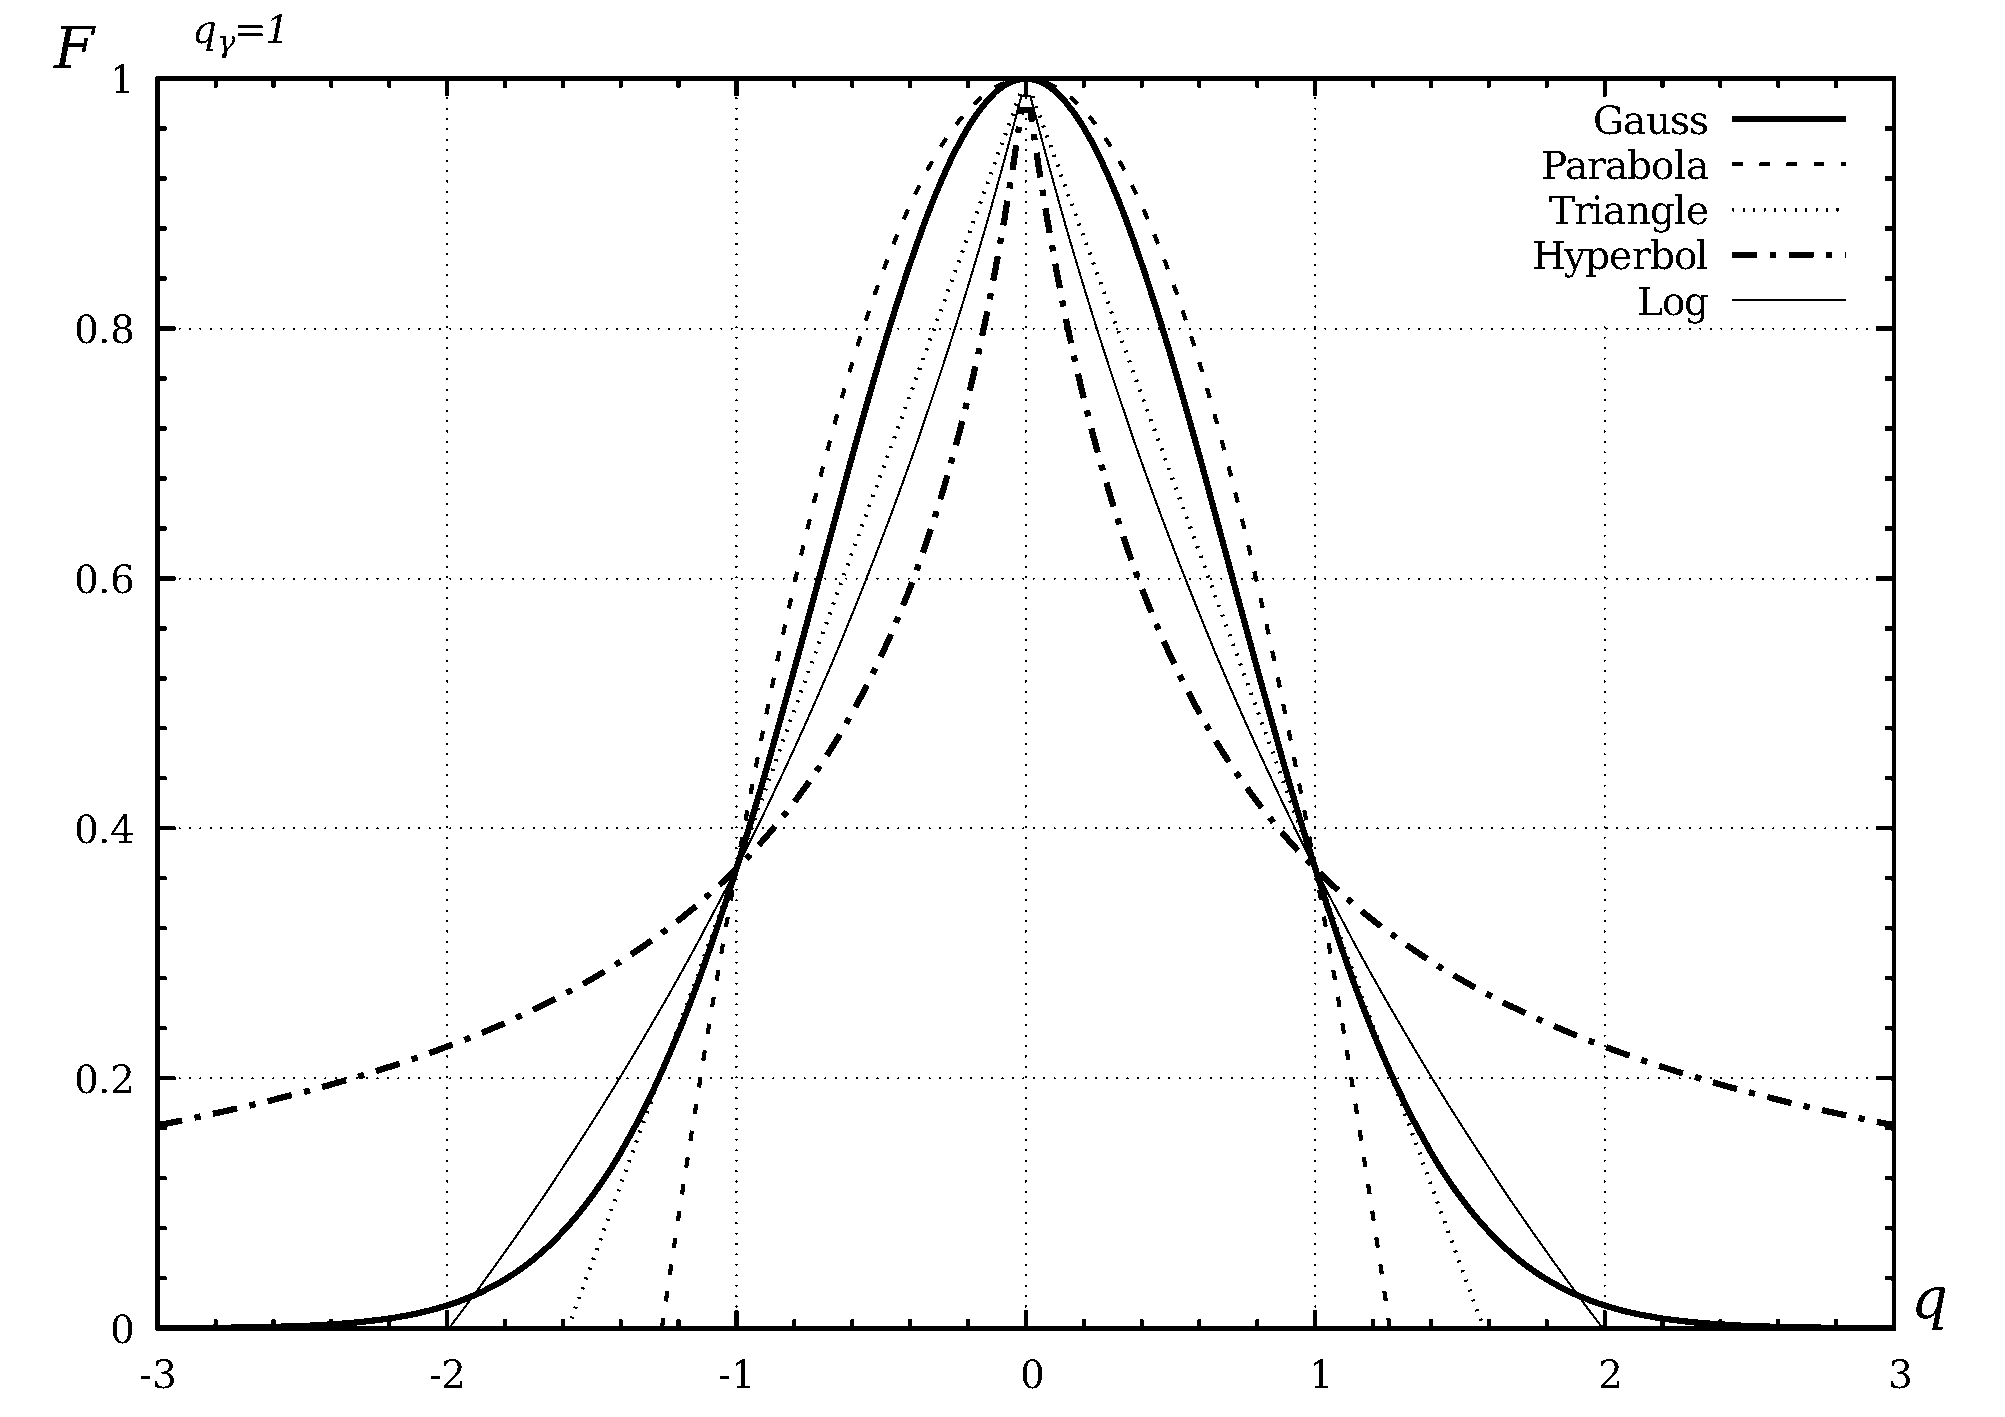
\includegraphics[width=45\TW]{p/F_types.png} }
  \caption{Функции качества идентификации (\ref{atu:eq:F_gauss})--(\ref{atu:eq:F_log})}
  \label{atu:f:F_types}
\end{figure}


% }}}2


\section{Структура поисковых систем}  % {{{1


Введём необходимые для дальнейшего изложения определения.

Определение: \textbf{поисковый агент} --- это динамическая система, получающая выходной ($x(t)$),
и, при необходимости входной сигнал ($u(t)$) от одной или нескольких моделей,
величину критерия идентификации, определённую для объекта $q_o(t)$,
может быть обмениваясь информацией с другими элементами поисковой системы,
на основании значения критерия идентификации
реализующая алгоритм настройки параметра модели (моделей)
таким образом, чтобы обеспечить идентификацию заданного параметра.


Определение: \textbf{координатор поиска} --- это динамическая система, получающая информацию
от поисковых агентов, и на основании этой информации определяющая
$p_\mathrm{id}(t)$ --- искомую величину идентифицируемого параметра.
Помимо этого, координатор может, на основании этой же информации,
управлять процессом адаптации всей поисковой системы.

Таким образом, система идентификации состоит
из множества агентов, и множества координаторов поиска,
совместно решающих задачу идентификации.

За исключением иерархических систем идентификации,
чаще всего используется один координатор поиска.

В простейшем случае, когда используется один поисковый агент,
обязанности агента и координатора могут быть совмещены.
Если отбросить этот вырожденный случай,
наиболее простой является ``плоская'' структура системы идентификации~(рис.~\ref{atu:f:agents_flat}).
При этом координатор единообразно получает информацию от всех поисковых агентов,
и, при необходимости, управляет ими.

\begin{figure}[htb!]
\begin{center}
../../p3/p/agents.pgf
\end{center}
\caption{Мультиагентная система идентификации с плоской структурой}
\label{atu:f:agents_flat}
\end{figure}

В более сложных случаях может использоваться иерархическая структура,
при этом каждый элемент, за исключением первого и последнего
уровня, служит как источником информации для последующего
уровня, так и координатором для предыдущего. При этом элемент
может как иметь непосредственно управляемую модель,
то есть выполнять роль агента, так и довольствоваться ролью промежуточного
координатора.

Некоторые конфигурации агентов и координаторов
в настоящее время практически применяются,
может быть под другими обозначениями и для других задач,
некоторые введены впервые.
Рассмотрим некоторые конфигурации.

\textbf{ Рой } --- множество агентов, обеспечивающее идентификацию за счёт
сосредоточения максимального количества агентов
в области предполагаемого максимума функции качества или же
заданного значения критерия. \Cmt{ref}.
Обычно --- три составляющие поведения
(движение о оцениваемому локальному экстремуму, --- к глобальному, случайная составляющая).

\Cmt{define}

\Cmt{Для сравнения требуется и это промоделировать.
Достаточно накладно --- надо много агентов. Как вариант --- добавить вручную агентов вблизи
экстремума.}

Достоинством данного подхода является простота алгоритмов,
которые должны быть реализованы агентами.
Недостатки --- требуется избыточное количество агентов.
Значительная часть агентов, находящихся вблизи экстремума,
практически не приносит информации. Роевые
алгоритмы (как и их прообразы в живой природе) ориентированы
для увеличения добычи ресурсов, а не информации. \Cmt{link}.
Также недостатком можно считать необходимость
получения информации от координатора (а именно, значение $p_\mathrm{id}$)
каждым агентом для возможности определения его динамики.

\textbf{ Строй } --- множество агентов, расположение которых,
и если необходимо, смещение, задаётся
единообразным образом.
Отсутствует индивидуальная динамика каждого агента.
Неподвижный строй образует \textbf{сетку},
как равномерно распределённую по пространству параметров,
так и нет.

Сложность алгоритмов, реализуемая каждым агентом в этом случае,
проще, чем в случае роя. Более того, передача информации от
координатора (в данном случае ``командира'') к агенту
является необязательной.
Тем не менее, возможности как адаптации,
так и просто повышения точности идентификации
у данного подхода сильно ограничены.

\textbf{ Ансамбль } --- множество агентов, обеспечивающее идентификацию за счёт
распределения агентов таким образом, который обеспечивает как
точность идентификации за счёт ограниченного скопления агентов
в областях предполагаемых максимумов, так и оперативное переключение
на другие области при изменении параметров за счёт недопущения
неоправданной скученности агентов.

Возможно применение систем идентификации с структурами и поведением более высокого уровня,
но в данной работе они не рассматриваются.

В данной работе основное внимание уделяется именно
поисковым структурам типа ``ансамбль''.
Очевидным недостатком данного подхода является
относительная сложность алгоритмов, реализуемая поисковыми агентами.


% }}}1


\section{Свойства, параметры и алгоритмы работы поисковых агентов}  % {{{1 -----------

\subsection{Задачи, входные и выходные сигналы поисковых агентов} % {{{2 ------------

В соответствии со своим определением,
один поисковый агент может управлять как одной моделью (рис.~\ref{atu:f:agent1}, \ref{atu:f:agent1q}),
так и несколькими (рис.~\ref{atu:f:agent2}).
При этом он может использовать информацию,
как полученную непосредственно от других агентов,
так и вычисленную в результате обработки данных на других уровнях системы идентификации.

\begin{figure}[htb!]
\begin{center}
% vi:syntax=tex
\begin{tikzpicture}
  \bXStyleBloc{semiboldline,inner sep=2pt};
  \bXLineStyle{medline};
  % --- U
  \bXInput{U};
  % --- M
  \bXBlocL[2.0]{M}{$\mathbf{M}_i$}{U};
  \bXLink[$u(t)$]{U}{M};
  % --- Q
  \bXBloc[3.5]{Q}{$q(t)$}{M};
  \path (Q.east) ++(0.0,-1.0em) coordinate (Qqm);
  \path (Q.south west) ++(-0.3,-0.4) coordinate (BLKlb);
  \bXLink[$x_i(t)$]{M}{Q};
  % --- F
  \bXBloc[2.5]{F}{$F(q_o,q_{mi})$}{Q};
  \path (F.west) ++(0.0,-1.0em) coordinate (Fqm);
  \path (F.west) ++(0.0,+1.0em) coordinate (Fqo);
  \path (Fqo) ++(-1.6em,+2.8em) coordinate (Fqoi) {};  % external input
  \draw[medlinep] (Fqoi) |- (Fqo);
  \node[below right] at (Fqoi) {$q_o(t)$};
  \bXLink[$q_i(t)$]{Qqm}{Fqm};
  % --- P
  \bXBloc[2]{P}{$P$}{F};
  \draw[boldline,<->] (P.north) -- +(0,0.8);
  \path (P.north east) ++(0.1,+0.4) node (BLKrt) {};
  \bXLink[$F_i(t)$]{F}{P};
  % -- output
  \bXOutput[2.8]{Po}{P};
  \bXLink[$p_i(t)$]{P}{Po};
  \bXOutput[1.0]{Por}{P};
  \fill(Por) circle[radius=0.05];
  \bXLineStyle{semiboldline};
  \bXReturn{Por}{M}{$p_i(t)$};
  % -- block
  \draw[subelem] (BLKlb) |- (BLKrt) |- (BLKlb);
  \bXStyleBlocDefault;
  \bXDefaultLineStyle;
  %
  \TikzAddPadding
  %
\end{tikzpicture}

\end{center}
\caption{Поисковый агент, использующий функцию качества $F$, и настраивающий параметр одной модели}
\label{atu:f:agent1}
\end{figure}


\begin{figure}[htb!]
\begin{center}
% vi:syntax=tex
\begin{tikzpicture}
  \bXStyleBloc{semiboldline,inner sep=2pt};
  \bXLineStyle{medline};
  % --- U
  \bXInput{U};
  % --- M
  \bXBlocL[2.0]{M}{$\mathbf{M}_i$}{U};
  \bXLink[$u(t)$]{U}{M};
  % --- Q
  \bXBloc[3.5]{Q}{$q$}{M};
  \path (Q.east) ++(0.0,-1.0em) coordinate (Qqm);
  \path (Q.south west) ++(-0.3,-0.4) coordinate (BLKlb);
  \bXLink[$x_i(t)$]{M}{Q};
  % --- P
  \bXBloc[2]{P}{$P$}{Q};
  \draw[infoline,<->] (P.north) -- +(0,0.8);
  \path (P.west) ++(0.0,-1.0em) coordinate (Pqm);
  \path (P.west) ++(0.0,+1.0em) coordinate (Pqo);
  \path (Pqo) ++(-1.6em,+2.8em) coordinate (Pqoi) {};  % external input
  \path (P.north east) ++(0.1,+0.4) node (BLKrt) {};
  \bXLink[$q_{i}(t)$]{Qqm}{Pqm};
  \draw[medlinep] (Pqoi) |- (Pqo);
  \node[below right] at (Pqoi) {$q_o(t) \qquad A_i$};
  %\bXLink[$F_i(t)$]{F}{P};
  % -- output
  \bXOutput[2.8]{Po}{P};
  \bXLink[$p_i(t)$]{P}{Po};
  \bXOutput[1.0]{Por}{P};
  \fill(Por) circle[radius=0.05];
  \bXLineStyle{semiboldline};
  \bXReturn{Por}{M}{$p_i(t)$};
  % -- block
  \draw[subelem] (BLKlb) |- (BLKrt) |- (BLKlb);
  \bXStyleBlocDefault;
  \bXDefaultLineStyle;
  %
  \TikzAddPadding
  %
\end{tikzpicture}

\end{center}
\caption{Поисковый агент, использующий критерий $q$, и настраивающий параметр одной модели}
\label{atu:f:agent1q}
\end{figure}


\begin{figure}[htb!]
\begin{center}
% vi:syntax=tex
\begin{tikzpicture}
  %\draw[hair,step=1.0em] (0,-3) grid (12.0,3.0);
  \bXStyleBloc{semiboldline,inner sep=2pt};
  \bXLineStyle{medline};
  % --- U
  \bXInput{U};
  \path (U.center) ++(2.5em,0.0em) coordinate (UxM);
  \draw (U.center) -- (UxM);
  \fill (UxM) circle[radius=0.05];
  \node[above right] at(U) {$u(t)$};
  % --- M0
  \bXBranchy[2]{UxM}{U0};
  %\fill[red](U0) circle[radius=0.05];
  \bXBlocL[2.0]{M0}{$\mathbf{M}_{i0}$}{U0};
  \bXLinkyx{UxM}{M0};
  % --- M1
  \bXBranchy[-2]{UxM}{U1};
  %\fill[green](U1) circle[radius=0.05];
  \bXBlocL[2.0]{M1}{$\mathbf{M}_{i1}$}{U1};
  \bXLinkyx{UxM}{M1};
  % --- A
  \path (M0.east) ++(3.1em,0.0em) coordinate (X0);
  \path (X0) ++(4.0em,0.0em) coordinate (P0S);
  \path (X0) ++(0.0em,-2.0em) coordinate (Alb);
  %\fill[red](Alb) circle[radius=0.05];
  \path (M1.east) ++(3.1em,0.0em) coordinate (X1);
  \path (X1) ++(4.0em,0.0em) coordinate (P1S);
  \path (X1) ++(0.0em,2.0em) coordinate (Alt);
  \path ( $0.5*(P0S) + 0.5*(P1S)$ ) coordinate(PS);
  \path ( $0.5*(X0) + 0.5*(X1)$ ) coordinate(QO);
  \draw[medlinep] (QO) ++(-3.2em,0em) -- (QO);
  \node[above left] at(QO) {$q_{o}(t)$};
  %\fill[green](Alt) circle[radius=0.05];
  \draw[boldline] (Alb) -- ++(4.0em,0.0em) |- (Alt) -- cycle; % ----- MAIN block
  \draw[medlinep] (M0.east) -- (X0); // % inputs: x_ix(t)
  \node[above right] at(M0.east) {$x_{i0}(t)$};
  \draw[medlinep] (M1.east) -- (X1);
  \node[above right] at(M1.east) {$x_{i1}(t)$};
  \draw[semiboldlinep] (P0S) -- ++(3.0em,0em) -- ++(0em,-3.0em) -| (M0.south); % -- out params
  \node[above right] at(P0S) {$p_{i0}(t)$};
  \draw[semiboldlinep] (P1S) -- ++(3.0em,0em) -- ++(0em,+3.0em) -| (M1.north);
  \node[above right] at(P1S) {$p_{i1}(t)$};
  \draw[medlinep] (PS) -- ++(4.0em,0em);
  \node[above right] at(PS) {$p_{i}(t)$};
  \path (PS) ++(-2.1em,0.0em) coordinate (AI);
  \node at(AI) {$\mathbf{A}_{i}$};
  %
  \TikzAddPadding
  %
\end{tikzpicture}

\end{center}
\caption{Поисковый агент, настраивающий параметры двух моделей}
\label{atu:f:agent2}
\end{figure}


Для упрощения обозначений величин, относящимся к различным агентам,
ведём обозначения. Если в данном контексте важно указание
индекса агента, то он указывается явно, например:
$F_{c,i}(t)$ --- значение функции качества для центральной (``c'') модели
агента с индексом ``i''. В тех случаях, когда
выбран конкретный агент, или когда обозначение применимо
ко всему множеству агентов, индекс можно упускать, например:
$p_e(t)$\label{atu:d:p_e} --- оценка значения параметра для текущего агента
или же для агентов вообще. Для обозначения ближайшей окрестности
агента используем такие обозначения:
``c'' --- ``center'' --- обозначает центральную или единственную
модель агента, или же относится к агенту в целом,
``l'' --- ``left'' --- обозначает, в зависимости от контекста,
или величину, относящуюся к предыдущему (по индексу) агенту,
или же первую модель (из двух или трёх), используемую
данным агентом,
``r'' --- ``right'' --- аналогично,
но в противоположную сторону в пространстве индексов.
В двумерном случае для второй координаты такую же роль
выполняются обозначения ``t'' --- ``top''
и ``b'' --- ``bottom''.
Если же необходимо указать индекс агента,
а величина относительно объекта
имеет обозначение ``c'', то эту часть обозначения
модно упустить, например:
$ p_i(t) \equiv p_{i,c}(t)$, $q_{i,c} \equiv q_{i}(t)$.
Все индексы одновременно опускать нельзя,
однако, в очевидных случаях можно опускать явную
зависимость от времени:
$ q_l(t) \equiv q_l$.
При необходимости, что величина относится к модели,
без указания конкретного индекса модели,
будем использовать индекс ``m'',
например $x_m$ --- выходной сигнал какой-то
(или же единственной) модели.

В случае, когда один агент настраивает несколько моделей,
или/и, если пространство параметров имеет размерность больше единицы,
вместо простого индекса $i$ могут применяется составные.

Каждый агент на основании как собственных измерений, так и информации,
полученных от других агентов, оценивает значение $p_e(t)$,
которое, по его данным, наиболее близко к $p_o(t)$.
Часть методов использует это представление неявным образом.
При этом, если значение $p_e$ выходит за пределы
значений параметров моделей, на основании которых
было получено это значение, то его следует считать сомнительным.
Степень ``уверенности'' в вычисленном значении $p_e$
обозначим $S_e \in [0;1]$ (surety).
В результате такие оценки в дальнейшем можно
как вообще исключать из рассмотрения, так и ограничить
его влияние на следующем уровне.
Или, как вариант --- можно ограничить область допустимых
значений $p_e$ значениями параметров используемых моделей.

Выходными сигналами агента являются:

\begin{itemize}

  \item
  $p_c(t)$ -- текущее значение параметра ;

  \item
  $p_e(t)$ -- текущее значение оценки параметра;

  \item
  $F_c(t)$ --- текущее значение функции качества
  (если используется одна  модель для агента, или же если агент каким-либо образом её усредняет
  или аппроксимирует в случае нескольких моделей);

  \item
  $q_c(t)$ --- значение критерия качества (аналогично предыдущей величине в случае нескольких моделей);

  \item
  $F_e(t)$ --- аппроксимированное значение функции качества
  в точке $p_e(t)$;

  \item
  $S_e(t)$ --- степень ``уверенности'' агента в полученном значении.

\end{itemize}

Некоторые из этих сигналов могут не использоваться в конкретной реализации
координатора поиска. Например, системы идентификации с одним агентом
практически не нуждаются в величине $S_e(t)$. Величина $q_c(t)$
достаточно редко используется при работе координатора.
Достаточно часто используются производные сигналы,
например $W(t) = F_c(t) S_e(t)$ (worthiness), совмещающий как локальную
уверенность агента в оценке $p_\mathrm{id}(t)$,
так и глобальную функцию качества.
Также указанные сигналы могут использоваться самим агентом непосредственно,
для определения собственной динамики.


Агенты, для оценивания величины $p_e$
могут использовать как значения критериев идентификации $q$
непосредственно, так и только значения функций качества,
соответствующие критериям.

Принципиальной разницы между конфигурациями
``один агент --- пара моделей''
и
``два агента, каждый управляет одной моделью'' нет.
Для определённости будем считать, что если поддерживается
постоянная разность между значениями параметров моделей,
или же эта разность определяется единообразно,
то это --- один агент. Если же разность
не определяется напрямую, и является следствием динамики каждой модели,
то имеет смысл говорить о паре агентов.

Тем не менее, при использовании пары моделей неоправданно много времени
тратится на перемещение поисковой пары, особенно при резких изменениях
идентифицируемого параметра. Поэтому, использование множества
поисковых агентов может кардинально уменьшить время идентификации.


Рассмотрим случай, когда каждый агент взаимодействует с двумя своими ближайшими соседями.
Для того, что бы обработать границы поисковой области есть несколько подходов,
которые требуют определения дополнительных моделей, использование которых
и обеспечивает как ограничение области поиска, так и единообразность
алгоритмов для агентов внутри.
В дальнейшем будем обозначать их индексами ``ll'' и ``rr''.

Для систем идентификации, использующих только один агент с двумя моделями,
это достаточно неплохой вариант.
Если же использовать несколько агентов, каждый с парой моделей,
то модели в этой системе будут использоваться нерационально.
Рассмотрим случай, когда значения параметров моделей распределены в пространстве
параметров последовательно, и значение параметра, соответствующее $q_o$ лежит между значениями
параметров пары соседних моделей.
При этом, если пара моделей принадлежит одному агенту, то он,
а следовательно, и вся система идентификации может достаточно точно
оценить значение $q_o$. Если же модели этой пары
принадлежат разным агентам --- то нет.

Для того, что бы нивелировать этот недостаток,
попробуем создать систему идентификации,
в которой количество моделей равно количеству агентов,
не считая, может быть, дополнительных моделей на границе рабочей области.

% TODO: really define!!!!!!!!!!!!!


Первый из подходов реализуется наиболее простым способом
и практически не требует затрат.
В этом случае для единообразия множество моделей дополняется двумя
(в одномерном случае) неподвижными псевдомоделями (fake models).
Для псевдомоделей считаем $  F_{ll} = F_{rr} = 0$,
а координаты выбираются за пределами рабочего диапазона поиска.
Применение этого подхода наиболее оправданно для агентов,
вычисляющих значение $p_e$ с помощью функции качества.
При этом, платой за меньшие вычислительные затраты
является появление ``сжимающего'' воздействия на весь ансамбль в целом.
Системы с агентами, которые используют для определения $p_e$ непосредственно значение критерия,
не могут напрямую воспользоваться этом подходом,
так как нулевому (или близкому к нулевому) значению функции качества
обычно соответствует неограниченное множество значений критерия.

Второй подход отличается применением неподвижных настоящих моделей
на границе рабочей области. При этом, агенты, соседствующие с этими моделями,
могут использовать  значения как параметров, так и критериев этих
моделей естественным образом. Основным недостатком этого подхода
является дополнительный расход ресурсов для моделей на границе.
Также применение таких моделей может быть затруднительно тех случаях,
когда моделирование за пределами (или непосредственно на границе)
невозможно из-за нарушения устойчивости моделей.
Тем не менее, этот подход, с одной стороны,
позволяет корректно применять агентов, использующих $q$,
а с другой --- позволяет избавиться от ``сжимающего'' воздействия
при использовании агентов, использующих $F$.

Промежуточным вариантом является подход,
при использовании которого тоже используются
псевдомодели, но вместо нулевого значения
функции качества используется или каким-либо образом аппроксимированное
значение $F$, (применимо и к $q$), или полученное в результате
предварительного моделирования.


% }}}2



\subsection{ Способы определения искомого значения параметра одним агентом }  % {{{2

Первой из задач, стоящих перед агентом идентификации,
является определение $p_e(t)$ на основании
имеющихся данных, а также оценку уверенности $S_e(t)$
в полученном значении.

Системы поисковой и адаптивно-поисковой идентификации,
используемые для работы с обычными нелинейными динамическими системами,
в качестве исходных данных как для определения непосредственно
искомого параметра, так и для построения поисковой траектории
использовали непосредственно выходные сигналы объекта ($x_o(t)$) и модели~($x_m(t)$).
При этом явно или неявно использовалась функция качества.
Более того, при определённых условиях, с учётом
инерционных и усредняющих свойств системы идентификации
такой подход, неявным образом, использовал
один из энергетических критериев.

При идентификации систем хаотической динамики
использование критерия идентификации является обязательным.
Естественно, это применимо и для систем, не проявляющих
хаотическую динамику. При этом агент,
для выполнения своих задач, может использовать
как как само значение критерия, так и соответствующее ему
значение функции качества. Алгоритмы,
используемые агентами в этих случаях,
будут существенно отличаться. В первую очередь
это связано с тем, что чётный вид функций качества
вынуждает использовать для определения максимума
методы, характерный для систем экстремального управления.

\Cmt{TODO: Невозможность точной аппроксимации, ошибки измерения, близость к линейно при близости агентов }




\paragraph{Демонстрационная задача}

Для демонстрации способов определения поисковым агентом
величины $p_e$ в стационарном или квазистационарном случае
введём следующую искусственную зависимость $q(p)$:
%
\begin{equation}
  q_\mathrm{dem}(p) = q_{00} + c_\mathrm{lin} \tilde{p} + c_\mathrm{s1} \sin( \pi \tilde{p} ) + c_\mathrm{s2} \sin( 2 \pi \tilde{p} ) + c_\mathrm{s20} \sin( 20 \pi \tilde{p} ),
  \label{atu:eq:q_dem}
\end{equation}
%
где $q_{00}$, $c_\mathrm{lin}$, $c_\mathrm{s1}$, $c_\mathrm{s2}$, $c_\mathrm{s20}$
--- коэффициенты, позволяющие
настроить эту зависимость для проверки заданного аспекта поведения агента,
$ \tilde{p} = \frac{p - p_{\min}}{\Delta p} $ --- обезразмеренный параметр.
При этом $\tilde{p} \in[0;1]$, $c_\mathrm{lin} \ne 0$ определяет линейную часть зависимости,
$c_\mathrm{s1}$ и $c_\mathrm{s2}$ определяют нелинейную часть, имеющую характерный масштаб
порядка рабочего диапазона $p$,
а $c_\mathrm{s20}$ определяет высокочастотную составляющую этой зависимости.
Если $c_\mathrm{s1} = 0$, $c_\mathrm{s2}=0$, $c_\mathrm{s20}=0$,
то задача определения $p_e$ становится тривиальной,
но такой случай также является полезным для анализе поведения агента.

В дальнейшем будем использовать эти обозначения при описании
различных режимов работы методов идентификации, а также
при моделировании тестовых задач.

Рассмотрим возможные способы определения $p_e$ для агентов,
использующих как критерий идентификации непосредственно,
так и функции качества.




\subsection{Методы агентов, использующих значения критерия }  % {{{2

Неподвижный агент, использующий для своей работы только одну модель,
и, соответственно, характерное для неё значения критерия,
практически не имеет самостоятельного смысла. Реальная польза от такого агента
может быть только в том случае, когда координатор
каким-то образом смог оценить зависимость $q(p)$ целиком,
и передал или эту зависимость агенту, или по его запросу вычисляет $p(q)$.
Очевидно, что в таком случае никакие поисковые агенты не нужны,
и можно просто вычислить $p(q_o)$.

Если агент, использующий одну модель является подвижным,
то он может оценить своё положение, используя историю.
\Cmt{TODO: more}

Рассмотрим случай, когда один подвижный агент и получает данные с двух моделей,
$ \mathbf{M}_{il}$ и
$ \mathbf{M}_{ir}$,
и управляет ими единообразным образом, например
выдерживая постоянное расстояние $\Delta p$ между ними в пространстве параметров.
В этом случае он может оценить, какая из моделей ближе по критерию
к объекту, и оценить положение $p_o$. \Cmt{TODO: Limit.}

Рассмотрим группу из трёх агентов:
$\mathrm{A}_l$,
$\mathrm{A}_c$,
$\mathrm{A}_r$.
Агент $\mathrm{A}_c$ со значением параметра $p_c$
сам определяет величину $q_c$,
от соседних агентов получает значения
$p_l$, $q_l$, $p_r$, $q_r$.
Будем считать, что динамика агентов определена так,
что $p_l(t) < p_c(t) < p_r(t) \; \forall t$.
Система идентификации обеспечивает каждого
агента значением $q_o$. С учётом всего вышеперечисленного,
задача определения $p_e$ заключается в нахождении такого $p$,
которое соответствует пересечению неизвестной кривой,
заданной тремя точками, с прямой $q=q_0$.
Формально, с учётом введённых ограничений,
три точки однозначно определяют параболу.
Однако, применение параболической аппроксимации в условиях
высокого уровня помех чаще всего неоправданно. Более того,
в этом случае потребуется дополнительная логика как для
выбора подходящего корня, так и для определения
``уверенности'' в полученном решении. Поэтому, будем рассматривать
линейное приближение с анализом полученной конфигурации.

Рассмотри возможные конфигурации в порядке,
обеспечивающем непротиворечивость алгоритма.

\paragraph{Случай 1.}
Это особый случай, когда значение $p_c$ агента
достаточно хорошо совпадает с искомым значением.
Понятие ``достаточно хорошо'' в данном случае определяется
поставкой задачи, и данном случае задаётся предельным значением
функции качества: $F_c > F_{\mathrm{good}}$, где $F_{\mathrm{good}}$
выбирается достаточно близко к единице.
При этом считаем: $p_e = p_c$,
$S_e = 1$, т.е. агент полностью ``уверен''
в полученном значении $p_e$.

Практически, для нескольких агентов может одновременно
может выполнится данное условие, и
дальнейшее определение $p_\mathrm{id}$ в этом противоречивом случае
возлагается на координатора поиска. Если данная
ситуация в процессе поиска случается достаточно редко,
то это, как правило, не нарушает общую динамику поиска.
Если же этот случай проявляется достаточно часто,
то это свидетельствует о грубых просчётах
при синтезе системы идентификации.
Например, такое поведение может вызвать применение
критерия, неподходящего для данной задачи,
или же предельно заниженная чувствительность функции качества.

Следует отметить, что в этом случае у агента нет необходимости
анализировать значения, полученные от соседних агентов.
Это позволяет избежать ряда ситуаций, в которых
алгоритм поиска будет давать сбои, связанные неопределённостью
алгоритмов поиска в вырожденных случаях.
В первую очередь,
если $F_c \le F_\mathrm{good}$, то $q_o -q_c \ne 0$,
и можно применить следующие упрощающие преобразования:
%
\[
  \tilde{p}_l = p_l - p_c;
  \quad
  \tilde{p}_c = p_c - p_c = 0;
  \quad
  \tilde{p}_r = p_r - p_c;
  \quad
  \tilde{p}_e = p_e - p_c;
\]
\begin{equation}
  \tilde{q}_l = \frac{q_l-q_c}{q_c-q_o};
  \quad
  \tilde{q}_c = \frac{q_c-q_o}{q_c-q_o} = 1;
  \quad
  \tilde{q}_l = \frac{q_l-q_c}{q_c-q_o}.
  \label{atu:eq:q_agent_rel}
\end{equation}

С учётом этих обозначений определим оценку $\tilde{p}_e$
для каждого из участков независимо:
%
\begin{equation}
  \tilde{p}_{el} = \frac{\tilde{p}_l}{1-\tilde{q}_l},
  \quad
  \tilde{p}_{er} = \frac{\tilde{p}_r}{1-\tilde{q}_r}.
  \label{atu:eq:pr_ex}
\end{equation}

Случай точного равенства нулю знаменателя в этих выражениях соответствует
бесконечно далёкому расположению $p_e$, полной неуверенности в полученном решении
($S_e = 0$) и алгоритмически исключается.


\paragraph{Случай 2.}
Все значения $q_l$, $q_c$, $q_r$ лежат по одну сторону
сторону от прямой $q=q_o$,
что эквивалентно условию $\tilde{q}_l > 0  $ и $\tilde{q}_r > 0  $.
В этом случае известно,
что $p_e \notin [p_l, p_r]$, то есть по данным текущих трёх моделей
нет возможности достаточно уверенно определить $p_e$. Тем не менее,
задача оценить $p_e$ всё равно остаётся актуальной.
Если система идентификации использует только одного агента,
то значение $p_e$, пусть даже ненадёжное, необходимо для
определения динамики агента, и соответственно, смещении
его в сторону области, где оценка будет более обоснованной.
Если же используется мультиагентная система,
то полученное значение $p_e$ достаточно ограничить искусственно.

При анализе данного случая необходимо рассмотреть несколько
вариантов.

Вариант A. Центральная точка --- наилучшая~(рис.~\ref{atu:f:pq_2A}),
т.е $\tilde{q}_l > 1 $ и $\tilde{q}_r > 1  $.

\begin{figure}[htb!]
  \centerline{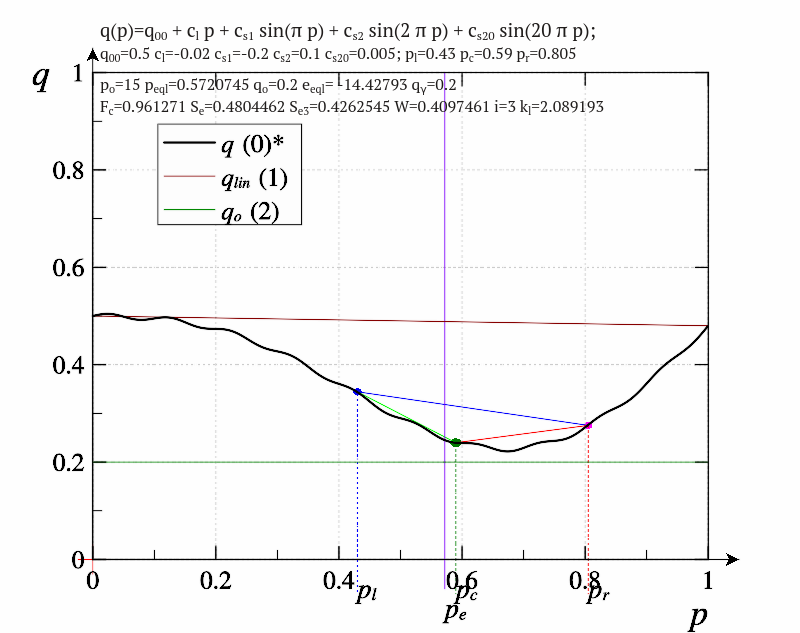
\includegraphics[width=50\TW]{p/pq_sin-p_pq_cgood.png} }
  \caption{Конфигурация точек, соответствующая случаю 2A}
  \label{atu:f:pq_2A}
\end{figure}

В этом случае происходит минимальная корректировка положения,
и уверенность в полученном решении невелика:
%
\begin{equation}
  \tilde{p}_e = 0.1 ( \tilde{p}_{el} + \tilde{p}_{er} ),
  \quad
  S_e = 0.2 \cdot
   e^{ \big( \frac{ 2 \tilde{p}_{e}}{(\tilde{p}_l + \tilde{p}_r)} \big)^2}.
  \label{atu:eq:pr_e_2A}
\end{equation}



Вариант B. Центральная точка --- промежуточная~(рис.~\ref{atu:f:pq_2B}).
Соответствует условию
$ ( \tilde{q}_l -1 ) \cdot ( \tilde{q}_r -1 ) < 0 $.

\begin{figure}[htb!]
  \centerline{
    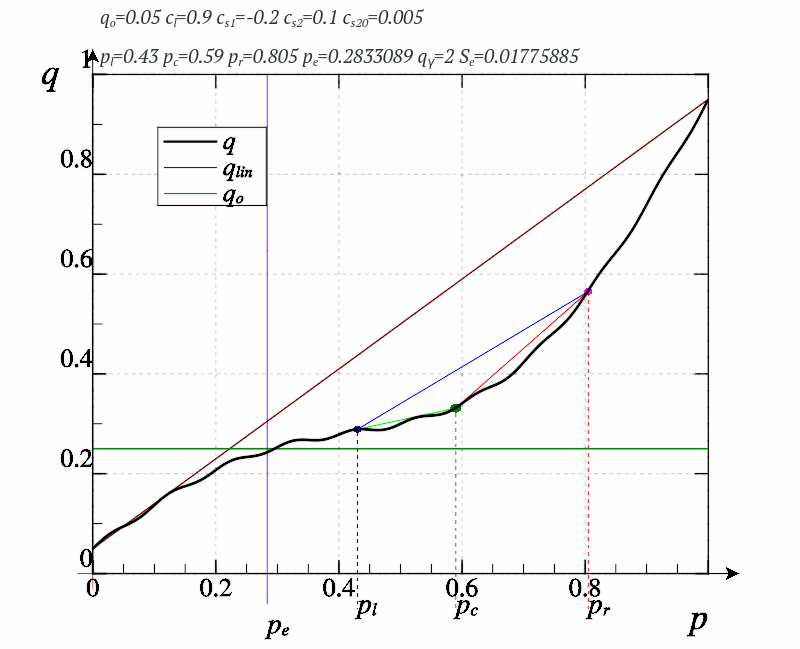
\includegraphics[width=49\TW]{p/pq_sin-p_pq_qo=025.png}
    \hfill
    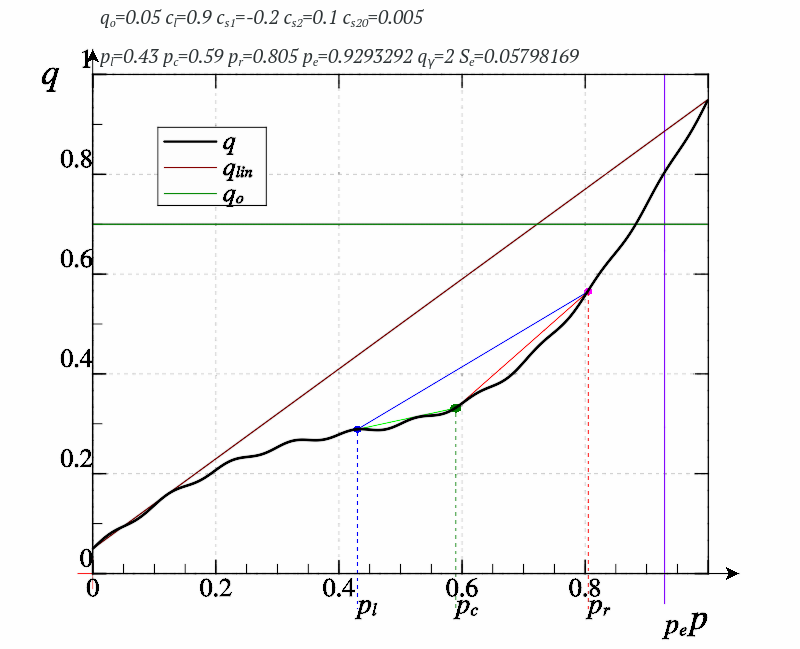
\includegraphics[width=49\TW]{p/pq_sin-p_pq_qo=070.png}
  }
  \caption{Конфигурации точек, соответствующие случаю 2B}
  \label{atu:f:pq_2B}
\end{figure}

В этом случае в качестве $\tilde{p}_e$ и $ S_e$ будем использовать
%
\begin{equation}
  \tilde{p}_e
  =
  \begin{cases}
    \tilde{p}_l, & \tilde{q}_l < \tilde{q}_r
    \\
    \tilde{p}_r, & \text{ otherwise}.
  \end{cases}
  ,
  S_e = 0.7 \cdot e^{(\frac{\tilde{p}_{e}}{\tilde{p}_b})^2}. % TODO: define p_b
  \label{atu:eq:pr_e2B}
\end{equation}


Вариант C. Центральная точка --- наихудшая~(рис.~\ref{atu:f:pq_2C}).

\begin{figure}[htb!]
  \centerline{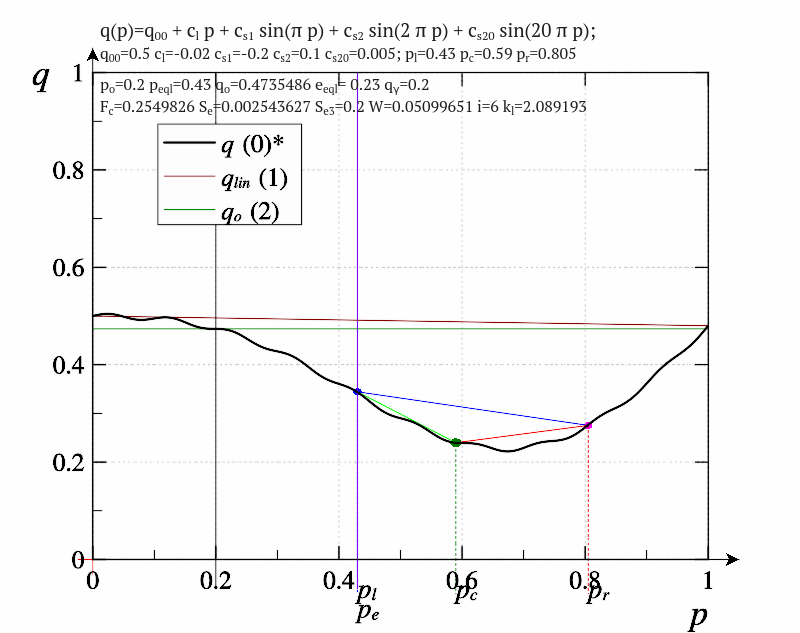
\includegraphics[width=50\TW]{p/pq_sin-p_pq_cbad.png} }
  \caption{Конфигурация точек, соответствующая случаю 2C}
  \label{atu:f:pq_2C}
\end{figure}

Этот вариант один из наименее благоприятных для определения $p_e$,
и этом случае можно поступить аналогично предыдущему случаю,
только с соответствующим штрафом в значении $S_e$.

\paragraph{Случай 3.}
Значения $q_l$ и $q_r$ лежат по одну сторону от прямой $q=q_o$,
а $q_c$ --- по другую, то есть существуют два корня в рассматриваемой области~(рис.~\ref{atu:f:pq_3}).
Это достаточно нетривиальный случай,
и при правильном критерии и идеальных условиях
встречаться не должен. Однако, в реальных условиях,
при наличии ошибок изменения и несовершенстве критерия
данный случай вполне возможен (пусть и достаточно редко), и требует отдельной обработки.

\begin{figure}[htb!]
  \centerline{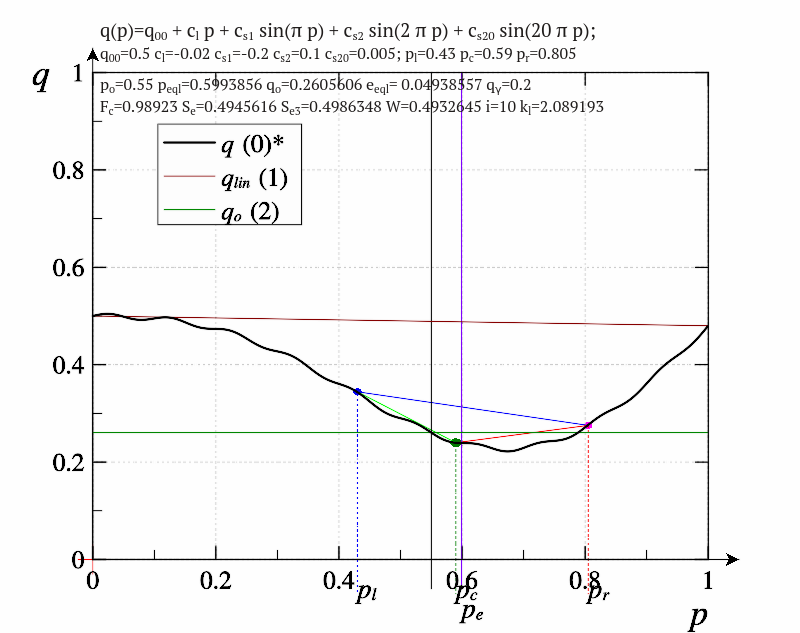
\includegraphics[width=50\TW]{p/pq_sin-p_pq_double.png} }
  \caption{Конфигурация точек, соответствующая случаю 3}
  \label{atu:f:pq_3}
\end{figure}

\Cmt{Action}

\paragraph{Случай 4.}
Две последовательные точки лежать по одну сторону от прямой $q=q_o$,
а оставшаяся --- по другую, то есть в рабочем диапазоне
существует только одно пересечение~(рис.~\ref{atu:f:pq_4}).


\begin{figure}[htb!]
  \centerline{
    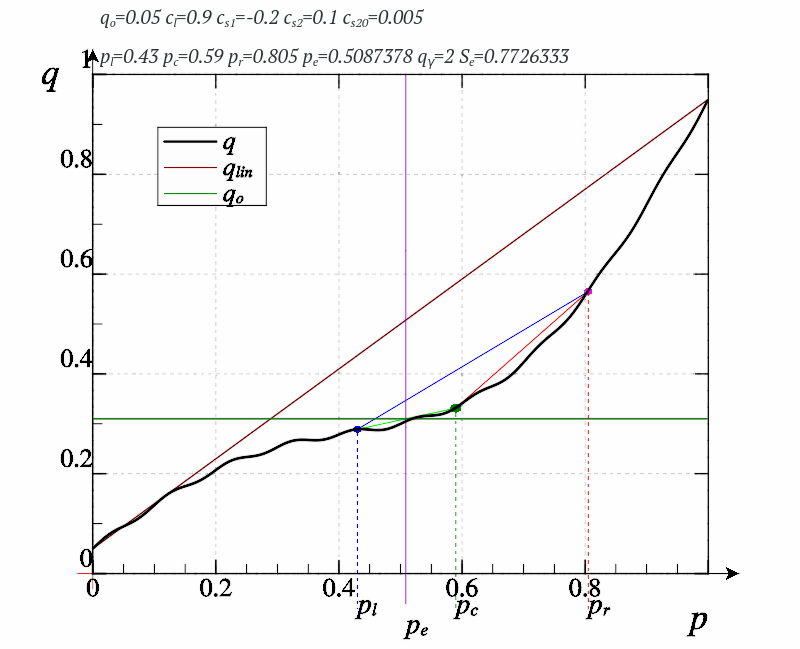
\includegraphics[width=49\TW]{p/pq_sin-p_pq_qo=031.png}
    \hfill
    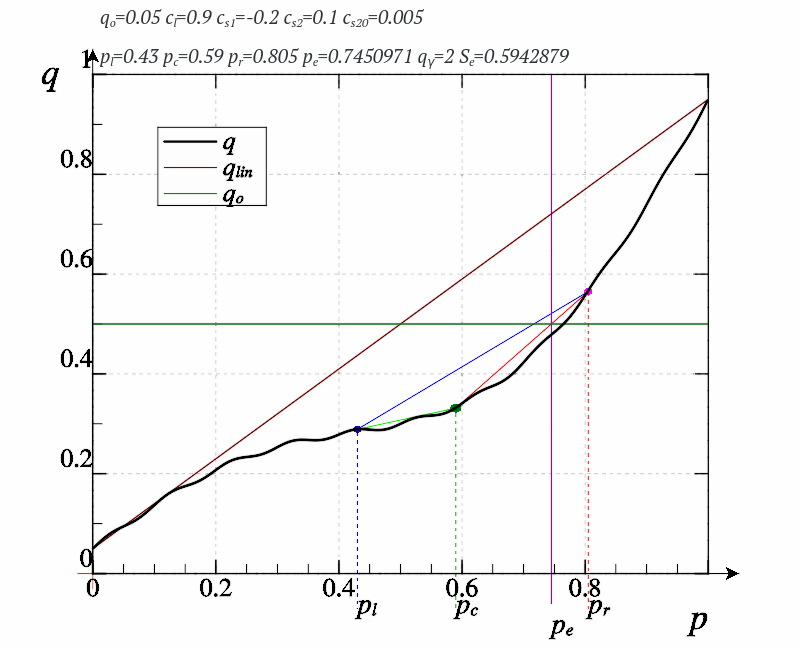
\includegraphics[width=49\TW]{p/pq_sin-p_pq_qo=050.png}
  }
  \caption{Конфигурации точек, соответствующие случаю 4}
  \label{atu:f:pq_4}
\end{figure}

В этом, самом благоприятном случае
\Cmt{Самое интересное пропущено!}

Описанный данными правилами способ
определения
$p_e$ в дальнейшем изложении будем обозначать $p_{eql}$\label{atu:d:p_eql}.

\paragraph{Учёт влияния оценки линейности зависимости $q(p)$}.

В предшествующих рассуждениях при вычислении коэффициента ``уверенности'' $S$
в расчёт принималось только расстояние от текущих значений параметров модели для $p_e$.
При этом не учитывалась возможность оценки линейности аппроксимации $q(p)$
по имеющимся данным. При этом оценка должна быть независима от изменения масштаба
как параметров, так и критериев, иметь удобную форму для дальнейшего
использования, и не требовать вычислений, сильно чувствительным к помехам измерений.

Так как в рассматриваемом случае один агент наблюдает значения $p$ и $q$
для трёх моделей, то оценить влияние нелинейных факторов он может
следующим образом. В первую очередь, по значениям, соответствующим крайним точкам
линейной интерполяцией оценивается значение $q_c$ (или же после нормализации --- $\tilde{q}_c$):
%
\begin{equation}
 q_{c,\mathrm{lin}}
  =
  \frac{  q_l \left( p_r - p_c \right) + q_r \left( p_c - p_l \right) }{p_r-p_l},
  \label{atu:eq:q_clin}
\end{equation}
%
\begin{equation}
  \tilde{q}_{c,\mathrm{lin}}
  =
  \frac{ \tilde{q}_l \tilde{p}_r - \tilde{q}_r \tilde{p}_l }{\tilde{p}_r-\tilde{p}_l}  .
  \label{atu:eq:qr_clin}
\end{equation}

Для обеспечения корректности и малой чувствительности полученных оценок
к ошибкам измерения следует обеспечить достаточное расстояние между соседними агентами.
Это требование необходимо учитывать при определении динамики агентов.
С другой стороны, проведении всех предыдущих оценках величины $p_e$
неявно предполагалось $\tilde{p}_l < 0$ и $\tilde{p}_r > 0$.
Следовательно, на начальном этапе работы метода случай чрезмерной близости агентов
детектироваться автоматически и обрабатываться отдельно особым образом.
Например, в этом случае имеет смысл принять $p_e = p_c$
при сохранении достаточно высоких значений $S$ --- если метод привёл
несколько агентов в малую окрестность одной точки, то
или точка действительно близка к искомой, или же весь метод
недостаточно пригоден для решения поставленной задачи.


Из полученных оценок $q_{c,\mathrm{lin}}$, $\tilde{q}_{c,\mathrm{lin}}$
сформируем следующие безразмерные коэффициенты, позволяющие оценить
нелинейность $q(p)$:
%
\begin{equation}
  k_l = 1 + \frac{|q_c - q_{c,\mathrm{lin}}}{|q_r-q_l|} ,
  \label{atu:eq:k_l1}
\end{equation}
%
\begin{equation}
  k_l = \frac{|\tilde{q}_c - \tilde{q}_{c,\mathrm{lin}}}{ |\tilde{q}_r-\tilde{q}_l|} .
  \label{atu:eq:k_l2}
\end{equation}

Данное представление $k_l$ было выбрано с целью непосредственного мультипликативного участия
% TODO: not so, it is a denominator - alike
этой величины в $S$, т.е. если $\tilde{q}_{c,\mathrm{lin}} \to \tilde{q}_c$,
то $k_l \to 1$, и есть основания полагать, что на расстояниях порядка $p_r-p_l$
оценка $p_e$ достаточно состоятельна. С другой стороны,
если $k_l \gg 1 $, то нелинейные эффекты в рассматриваемой области
преобладают над линейными, и оценку $p_e$  стоит рассматривать как недостоверную.

\Cmt{Correct $S$ definition}



% }}}2

\subsection{Методы агентов, использующих значения функции качества }  % {{{2

Единственный неподвижный агент,
использующий значение функции качества,
ещё более бесполезен (с точки зрения синтеза системы идентификации),
чем один неподвижный агент,
использующий значение критерия, так как в этом случае даже наличие
зависимости $q(p)$ не даёт возможности однозначно определить
значение параметра.
Он может сигнализировать о том, что в пределах
\(\tau\) модель была или не была достаточно адекватна
объекту.

% TODO: full rewrite,
\begin{figure}[htb!]
  \centerline{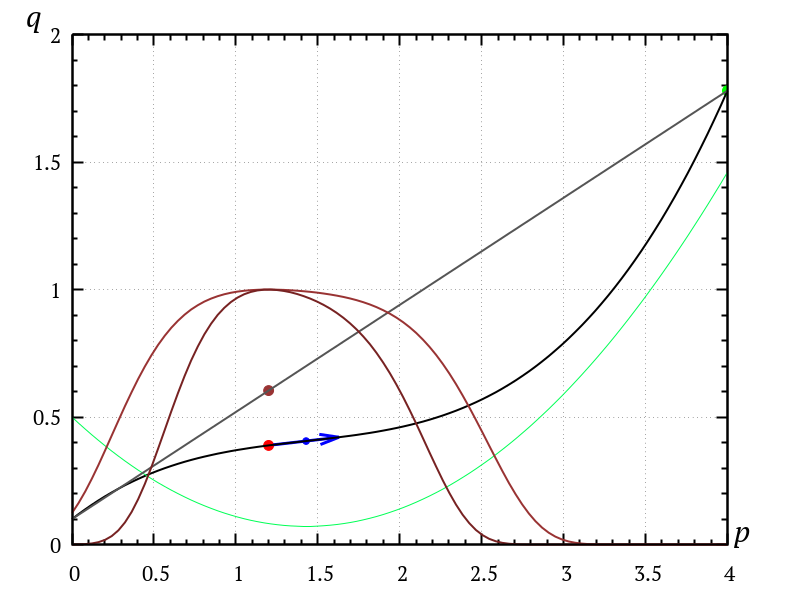
\includegraphics[width=0.6\textwidth]{pq_1x2.png} }
  \caption{ $q(p)$, $F(q(p))$, part1 }
  \label{atu:pq_1x2}
\end{figure}

\begin{figure}[htb!]
  \centerline{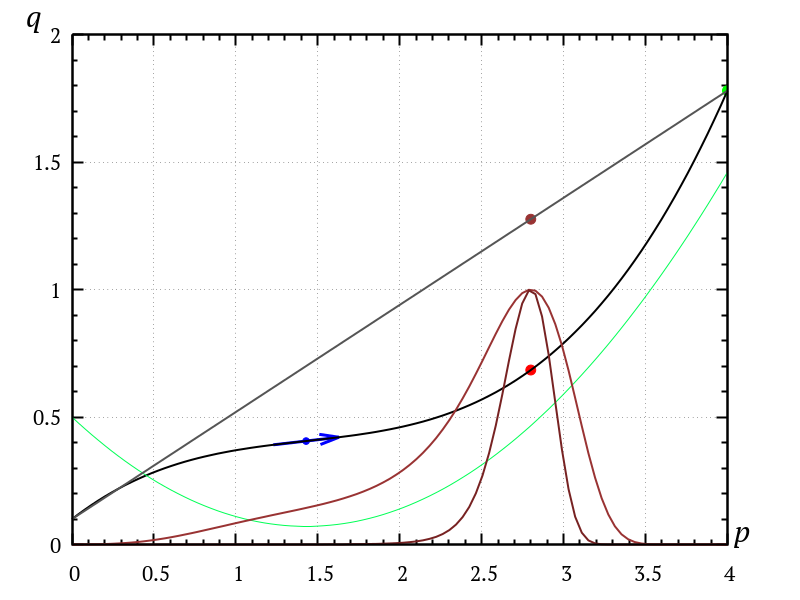
\includegraphics[width=0.6\textwidth]{pq_2x8.png} }
  \caption{$q(p)$, $F(q(p))$, part2 }
  \label{atu:pq_2x8}
\end{figure}

% }}}2


Наличие истории и возможность перемещаться дают возможность
построить систему идентификации и на одном агенте.
В качестве истории могут использоваться, в том числе,
динамические свойства идентифицируемого объекта
(оригинальный метод АПИ). Также могут быть
применены интегрирующие элементы агента идентификации
(синхронный детектор, \ldots).

В простейших случаях возможно построение системы идентификации
с одной моделью и, соответственно, одним поисковым агентом.
Примерами такого похода могут служить
метод синхронного детектора \cite{adopt_cont_sys}
и оригинальный адаптивно-поисковый метод \cite{mich_92}.
Применение одномодельных методов требует определённого механизма
сохранения истории процесса поиска, по крайней мере в пределах
одного поискового ``периода''. Это сильно ограничивает диапазон
применимости данных методов, в первую очередь --- из-за значительных
временных затрат на повторяющийся поиск.

Применение пары моделей \cite{atu_asau3} \Cmt{figure, or link to p1?}
(в этом случае имеет смысл говорить об одном поисковом агенте)
позволяет с меньшими временными затратами оценить градиент функции качества,
и, как следствие --- определить значение параметра. Также значительным преимуществом
такого подхода является меньшая скорость изменения параметров моделей.


Пара агентов, взаимодействующая между собой,
способна оценить градиент функции качества,
и, следовательно, обеспечить смещение в требуемом направлении.

С учетом глобальной информации возможна адаптация параметров пары.
В свою очередь, информация, полученная от пары может
использоваться для уточнения глобальных параметров.



Каждый поисковый агент, определяя величину $q_{i}(t)$, и получая $q_o(t)$,
вычисляет безразмерную функцию качества идентификации
$F(q_o,q_i)$. Как вариант, агент (или даже вся управляемая часть системы идентификации)
не имеет непосредственного доступа к критерию,
и получает собственно значения $F$.




Три соседних агента, взаимодействующие между собой,
способны не только оценить градиент функции качества в своей окрестности,
но и определить (опять же, оценочно) наличие там максимума.

В отличие от методов, использующих значение критерия непосредственно,
в этом случае нет возможности обрабатывать
каждую из пар точек ($p_l,p_c$) и ($p_c,p_r$) независимо.
По трём точкам вблизи  $M_{i}$
функция $F(p)$ аппроксимируется параболой, и абсцисса её вершины задаёт искомое
значение параметра. Сместим начало координат в точку
$ ( p_c, F_c ) $. Тогда
%
\[
  \tilde{p}_c = 0, \,
  \tilde{p}_l = p_l - p_c, \,
  \tilde{p}_r = p_r - p_c.
\]
%
\[
  \tilde{F}_c = 0, \,
  \tilde{F}_l = F_l - F_c, \,
  \tilde{F}_r = F_r - F_c.
\]
%
\[
  \left\{
    \begin{array}{l}
      a_2 \tilde{p}_l^2 + a_1 \tilde{p}_l  = \tilde{F}_l
      \\
      a_2 \tilde{p}_r^2 + a_1 \tilde{p}_r  = \tilde{F}_r
    \end{array}
  \right. .
\]
%
\[
  a_1 = \frac{\tilde{F}_r \tilde{p}_l^2 - \tilde{F}_l \tilde{p}_r^2 }
             { \tilde{p}_l^2 \tilde{p}_r  + \tilde{p}_l \tilde{p}_r^2 }.
\]
%
\[
  a_2 = \frac{\tilde{F}_r \tilde{p}_l - \tilde{F}_l \tilde{p}_r }
             { \tilde{p}_l^2 \tilde{p}_r  + \tilde{p}_l \tilde{p}_r^2 }.
\]

\begin{equation}
  \tilde{p}_e = - \frac{a_1}{2 a_2};
  \;
  p_e = p_c - \frac{a_1}{2 a_2}.
  \label{atu:eq:p_eFq}
\end{equation}


При этом, если
$ p_e \notin [ p_l, p_r ] $, или $ a_2 \ge 0 $, то значение $p_e$ искусственно
ограничивается этим диапазоном.

Определение $p_e$ по (\ref{atu:eq:p_eFq}) будем обозначать $p_{eFq}$.

\paragraph{Определение $p_e$ методом COG по значениям функции качества в 3 точках}

Достаточно простым и малозатратным с точки зрения вычислений
является метод оценивания $p_e$ методом COG (``Center of gravity'')
по значениям функции качества:
%
\begin{equation}
  p_e =
  \frac{p_l F_l + p_c F_c + p_r F_r}{ F_r + F_c + F_r}  .
  \label{atu:eq:p_eFc}
\end{equation}

Условие ограниченности оценки
$p_e \in [p_l;p_r]$ в этом случае выполняется автоматически.
Единственная сложность --- обработка особого случая для тех видов
$F(q)$, которые обращаются в ноль на удалении от центральной точки.
В этом случае знаменатель (\ref{atu:eq:p_eFc}) обращается в ноль,
в в качестве $p_e$ имеет смысл выбрать $p_c$.
Для тех видов функций качества, которые не принимают строго нулевых
значений, формально такой проблемы нет. Нем не менее,
данное состояние сильно подвержено влиянию помех измерения.

Для этого способа не представляется возможным
достаточно полезным способом определить величину $S$,
поэтому, для сохранения единообразия положим $S=1$.

Определение $p_e$ по (\ref{atu:eq:p_eFc}) в дальнейшем будем обозначать $p_{eFc}$.



% }}}2

\subsection{Оценка работоспособности и эффективности методов оценивания идентифицируемого параметра одним поисковым агентом}  % {{{2

Для определения работоспособности и свойств различных методов оценивания $p_e$
в контролируемых условиях без учёта динамики агентов, была выбрана следующая
тестовая задача: зависимость $q(p)$ определялась по (\ref{atu:eq:q_dem}),
$p_{\min}=20$, $p_{\max}=60$,
$q_{00}=7$, $c_\mathrm{lin}=-4.0$.
Изначальное расположение агентов равномерное, и искусственно  зафиксированное:
$p_l=30$, $p_c=40$,  $p_r=50$.

Значения коэффициентов
$c_\mathrm{s1}$, $c_\mathrm{s2}$, $c_\mathrm{s20}$
выбирались по одному из трёх наборов:
%
\begin{equation}
  c_\mathrm{s1} = 0.2, c_\mathrm{s2} = -0.4, c_\mathrm{s20} = 0.02,
  \label{atu:eq:q_dem_all}
\end{equation}
%
\begin{equation}
  c_\mathrm{s1} = 0, c_\mathrm{s2} = 0, c_\mathrm{s20} = 0.02,
  \label{atu:eq:q_dem_s20}
\end{equation}
%
\begin{equation}
  c_\mathrm{s1} = c_\mathrm{s2} = c_\mathrm{s20} = 0 .
  \label{atu:eq:q_dem_lin}
\end{equation}

При этом набор параметров (\ref{atu:eq:q_dem_all})
позволяет исследовать поведение ошибки идентификации при
влиянии как низкочастотных, так и высокочастотных
нелинейных компонент,
(\ref{atu:eq:q_dem_s20}) --- только высокочастотных,
а (\ref{atu:eq:q_dem_lin}) представляет собой
простейший линейный случай.
\Cmt{TODO: pic}

В первой серии вычислительных экспериментов
значение параметра объекта $p_o$
пробегало значения от $p_{\min}$ до $p_{\max}$
при фиксированном расстоянии между агентами $A = p_c - p_l = p_r - p_c$.
Это позволило оценить как интерполяционные (при $p_o \in [p_l,p_r] $),
так и экстраполяционные возможности методов. Так как
часть методов при определении $p_e$ использует значения
функции качества, то при проведении экспериментов
величина $q_\gamma$ также варьировалась.
Для метода $p_{eql}$ непосредственной зависимости от этой величины нет,
но для единообразия представленных результатов
все графики приведены как зависимости от $p_o$ и $q_\gamma$.
Все представленные графики, для удобства сравнения,
выполнены в одном масштабе и одной и той же проекции.
Масштаб по оси $Z$, использующейся для представления
модуля ошибки идентификации, был выбран $Z_{\max} = A/2 = 5$
для наглядного сравнения с расстоянием между агентами,
при этом величины, большие $A/2$ соответствуют
неоправданно большой ошибке, и находятся за пределами графика.




\begin{figure}[htb!]
  \centerline{
    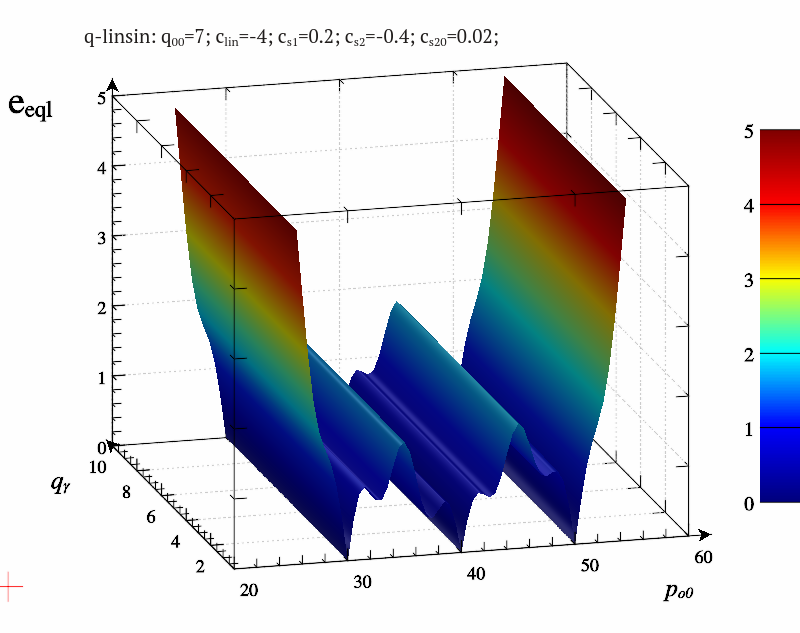
\includegraphics[width=0.32\textwidth]{p/qls_pe-p_po_qg_eql_all.png}
    \hfill
    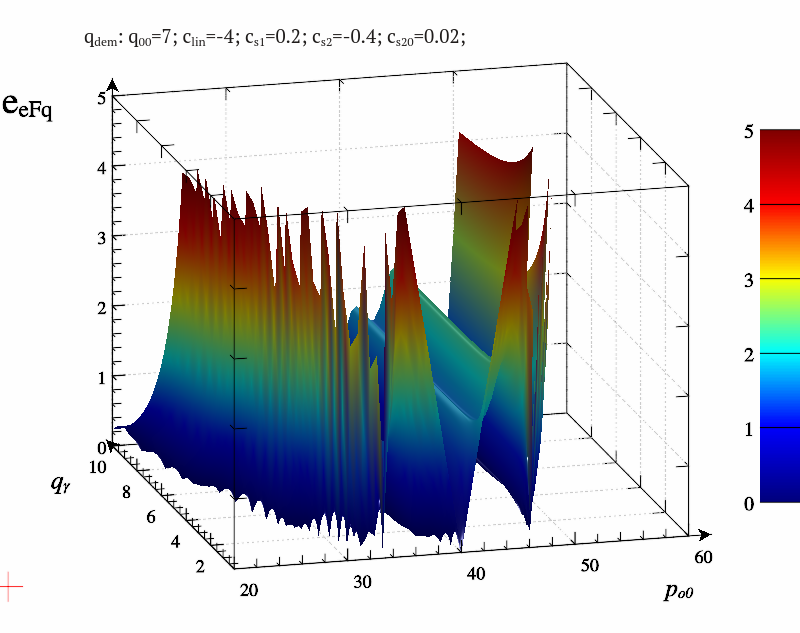
\includegraphics[width=0.32\textwidth]{p/qls_pe-p_po_qg_eFq_all.png}
    \hfill
    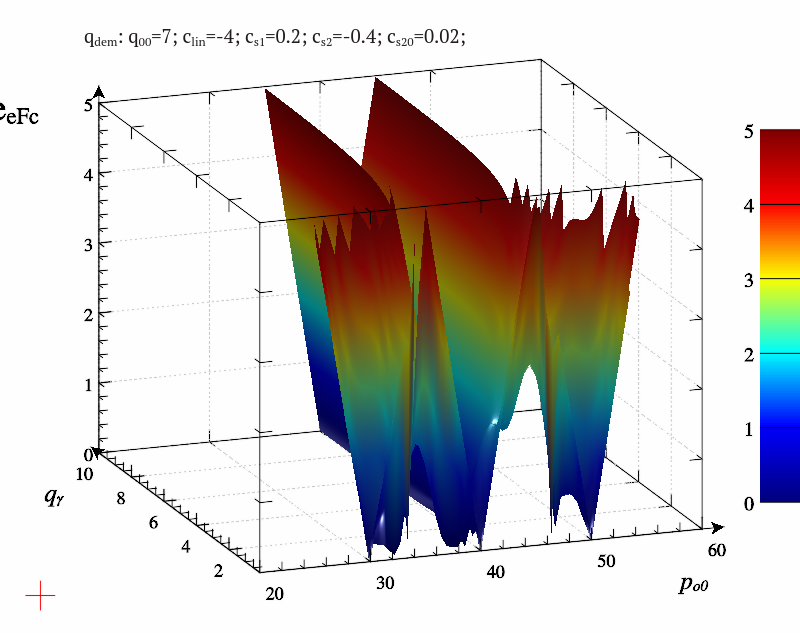
\includegraphics[width=0.32\textwidth]{p/qls_pe-p_po_qg_eFc_all.png}
  }
  \caption{Зависимости $e(p_o,q_\gamma)$ для методов $p_{eql}$, $p_{eFq}$, $p_{qFc}$ для условий (\ref{atu:eq:q_dem_all})}
  \label{atu:f:qsl_pe_po_qg_all}
\end{figure}


\begin{figure}[htb!]
  \centerline{
    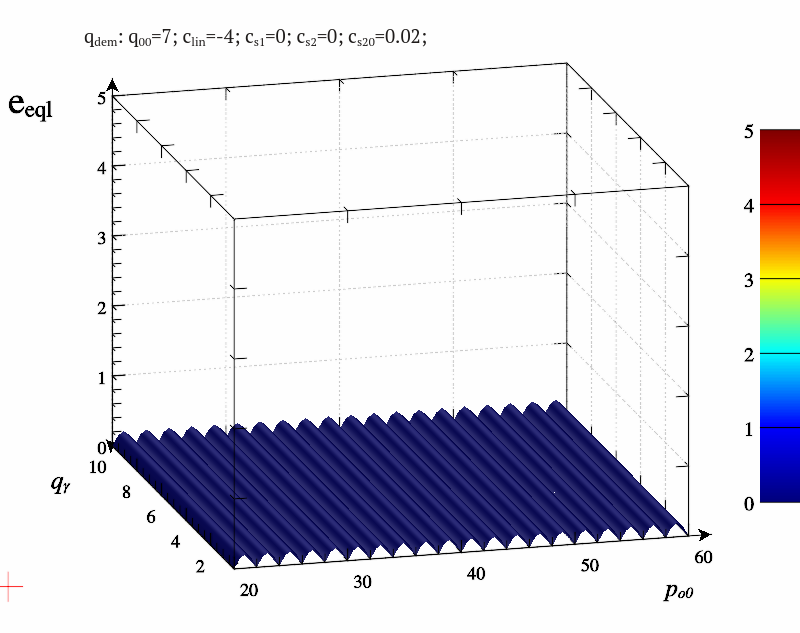
\includegraphics[width=0.32\textwidth]{p/qls_pe-p_po_qg_eql_s20.png}
    \hfill
    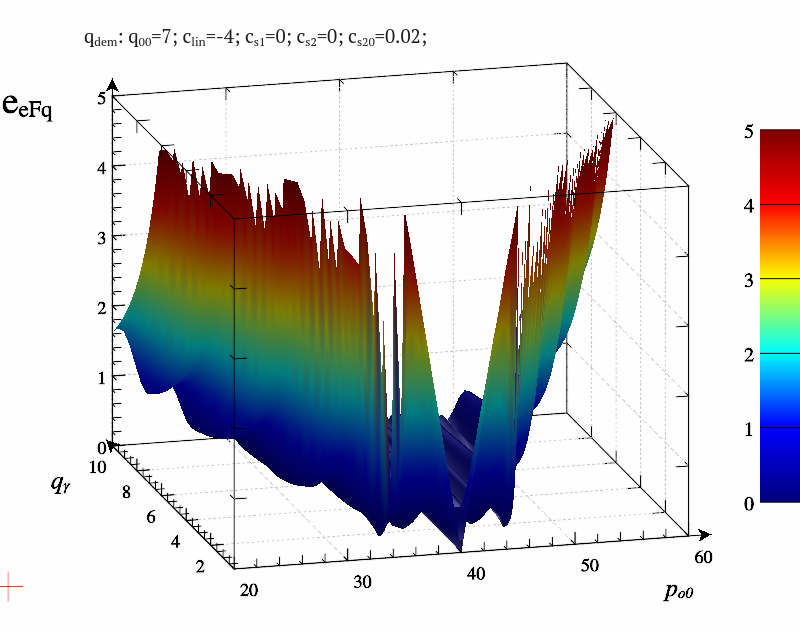
\includegraphics[width=0.32\textwidth]{p/qls_pe-p_po_qg_eFq_s20.png}
    \hfill
    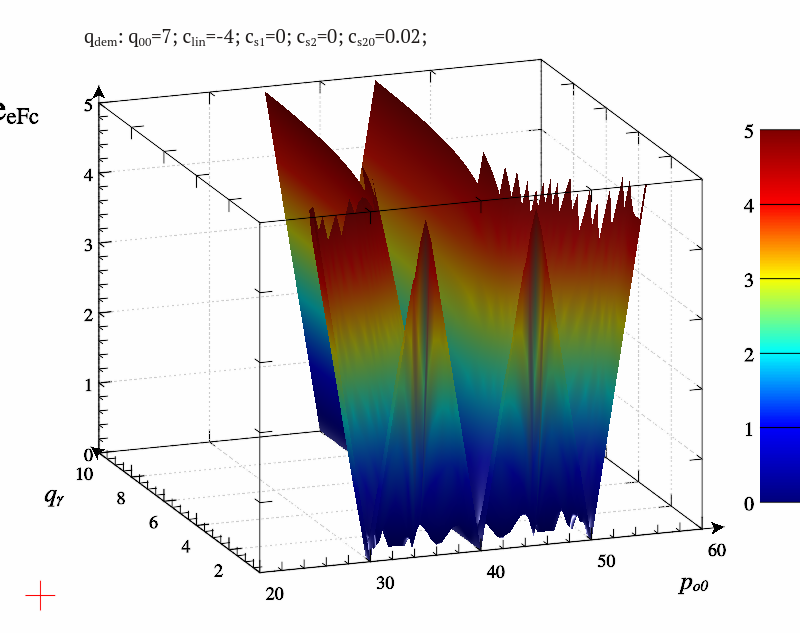
\includegraphics[width=0.32\textwidth]{p/qls_pe-p_po_qg_eFc_s20.png}
  }
  \caption{Зависимости $e(p_o,q_\gamma)$ для методов $p_{eql}$, $p_{eFq}$, $p_{qFc}$ для условий (\ref{atu:eq:q_dem_s20})}
  \label{atu:f:qsl_pe_po_qg_s20}
\end{figure}

\begin{figure}[htb!]
  \centerline{
    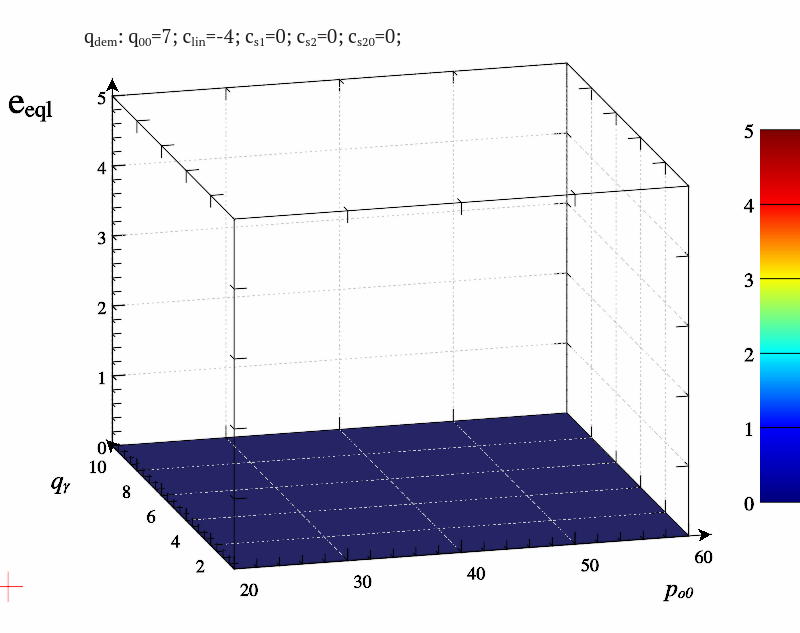
\includegraphics[width=0.32\textwidth]{p/qls_pe-p_po_qg_eql_lin.png}
    \hfill
    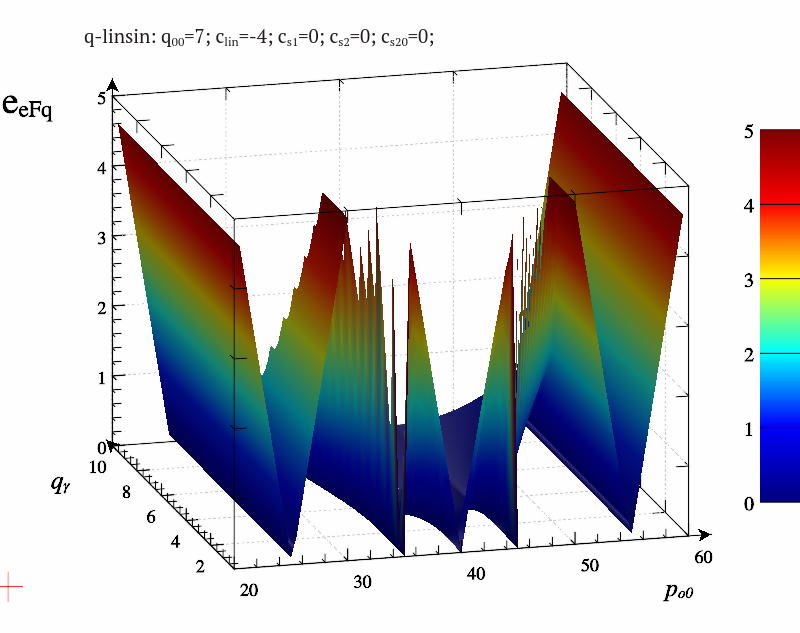
\includegraphics[width=0.32\textwidth]{p/qls_pe-p_po_qg_eFq_lin.png}
    \hfill
    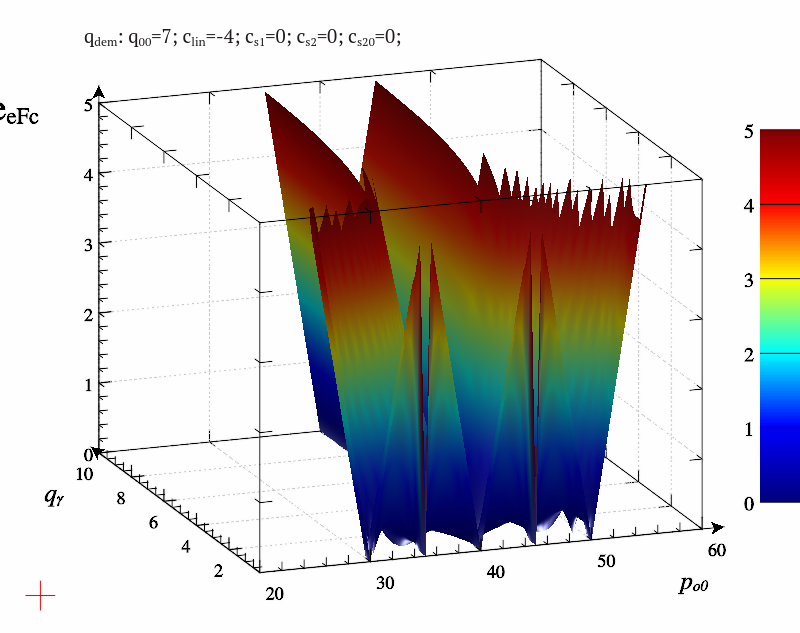
\includegraphics[width=0.32\textwidth]{p/qls_pe-p_po_qg_eFc_lin.png}
  }
  \caption{Зависимости $e(p_o,q_\gamma)$ для методов $p_{eql}$, $p_{eFq}$, $p_{qFc}$ для условий (\ref{atu:eq:q_dem_lin})}
  \label{atu:f:qsl_pe_po_qg_lin}
\end{figure}



\begin{figure}[htb!]
  \centerline{
    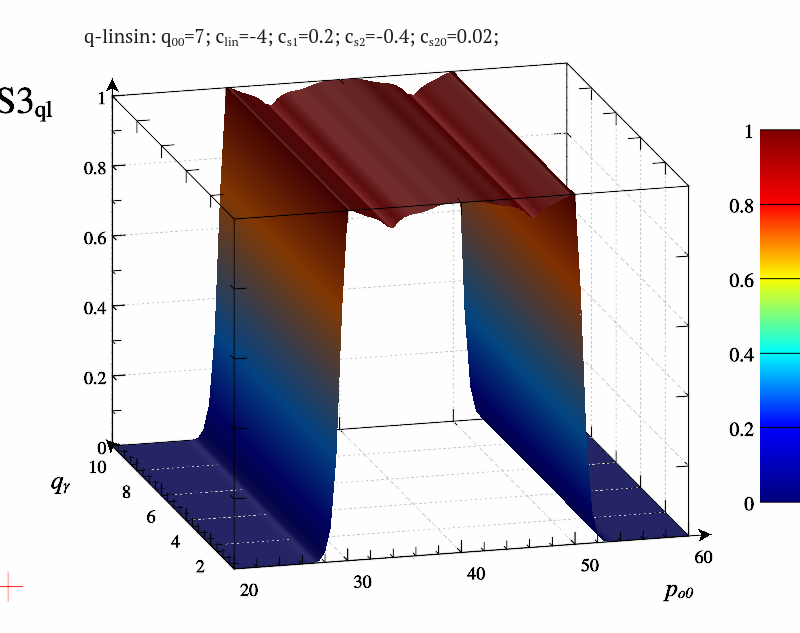
\includegraphics[width=0.32\textwidth]{p/qls_pe-p_po_qg_Sql_all.png}
    \hfill
    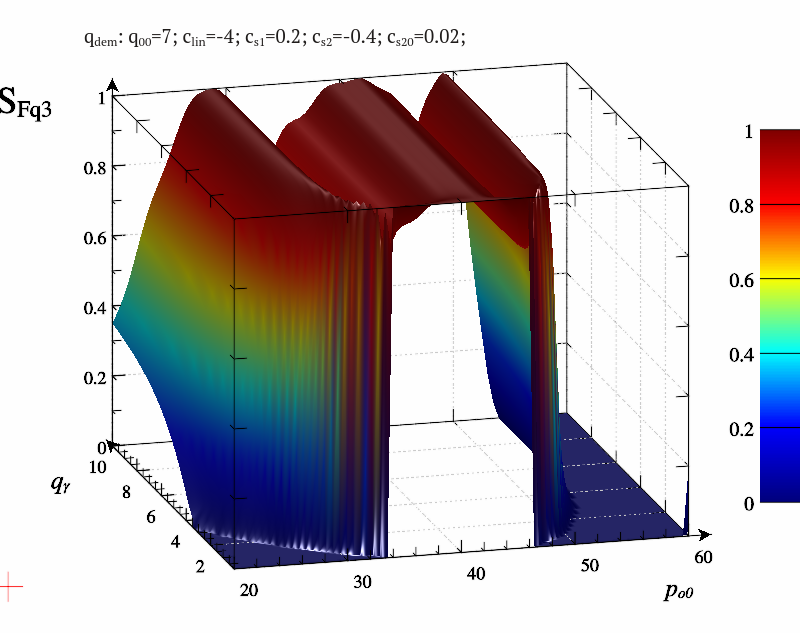
\includegraphics[width=0.32\textwidth]{p/qls_pe-p_po_qg_SFq_all.png}
    \hfill
    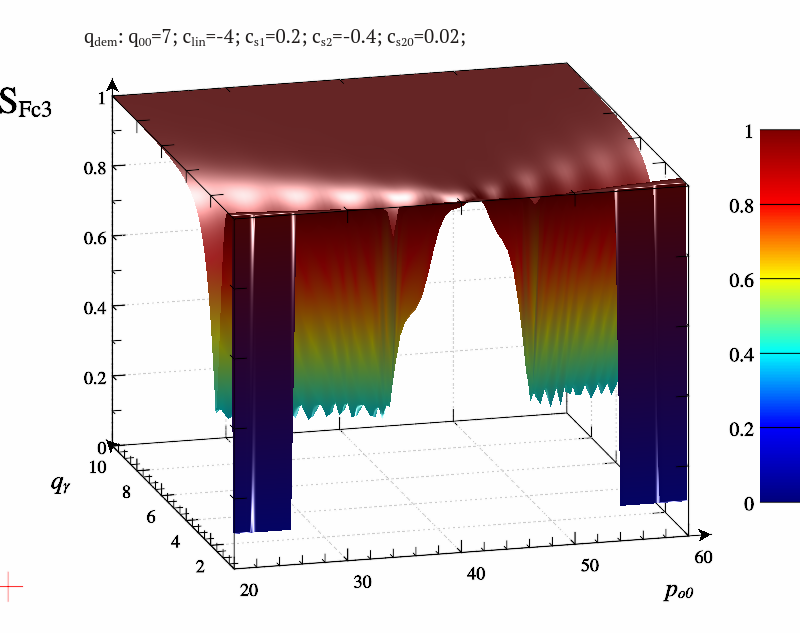
\includegraphics[width=0.32\textwidth]{p/qls_pe-p_po_qg_SFc_all.png}
  }
  \caption{Зависимости $S(p_o,q_\gamma)$ для методов $p_{eql}$, $p_{eFq}$, $p_{qFc}$ для условий (\ref{atu:eq:q_dem_all})}
  \label{atu:f:qsl_S_po_qg_all}
\end{figure}


\begin{figure}[htb!]
  \centerline{
    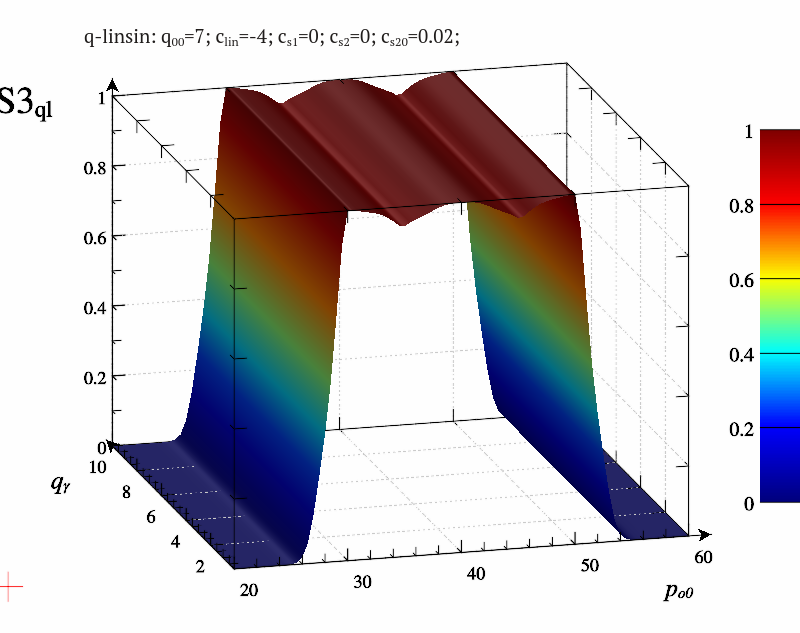
\includegraphics[width=0.32\textwidth]{p/qls_pe-p_po_qg_Sql_s20.png}
    \hfill
    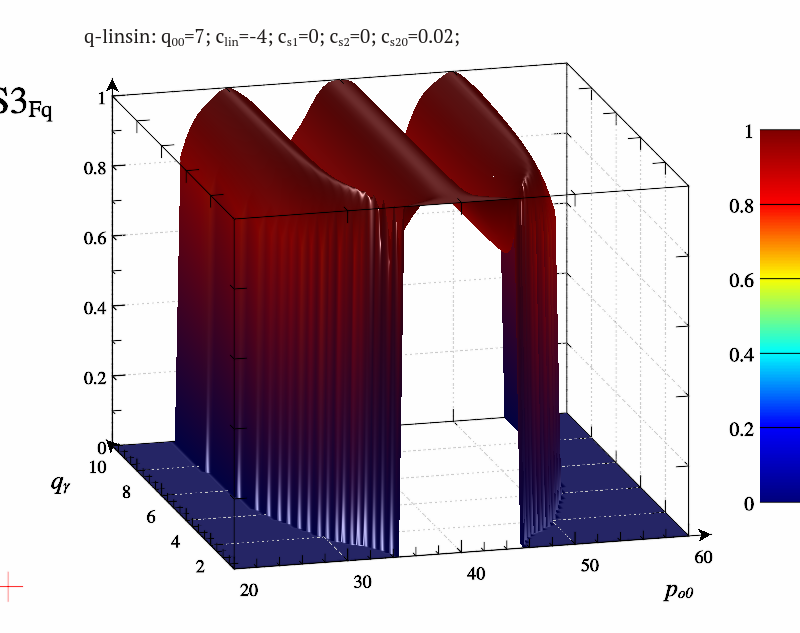
\includegraphics[width=0.32\textwidth]{p/qls_pe-p_po_qg_SFq_s20.png}
    \hfill
    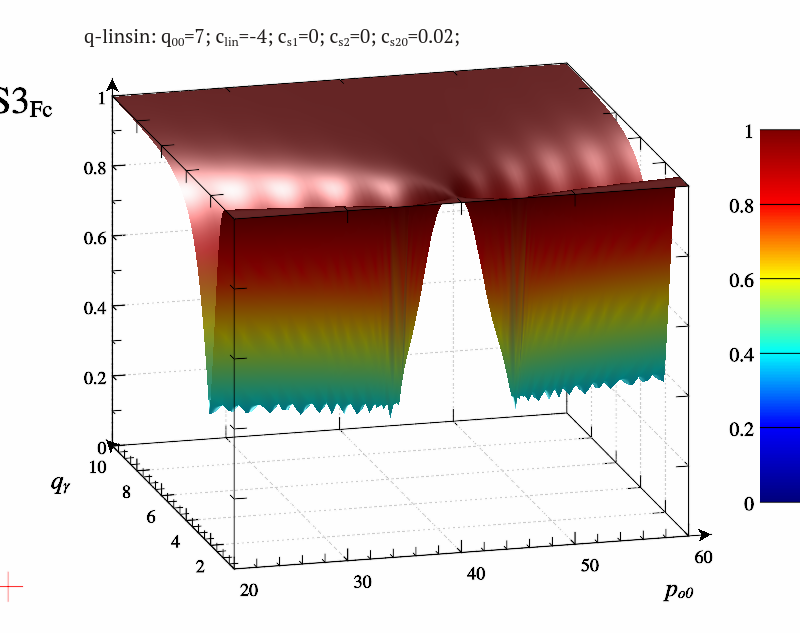
\includegraphics[width=0.32\textwidth]{p/qls_pe-p_po_qg_SFc_s20.png}
  }
  \caption{Зависимости $S(p_o,q_\gamma)$ для методов $p_{eql}$, $p_{eFq}$, $p_{qFc}$ для условий (\ref{atu:eq:q_dem_s20})}
  \label{atu:f:qsl_S_po_qg_s20}
\end{figure}

\begin{figure}[htb!]
  \centerline{
    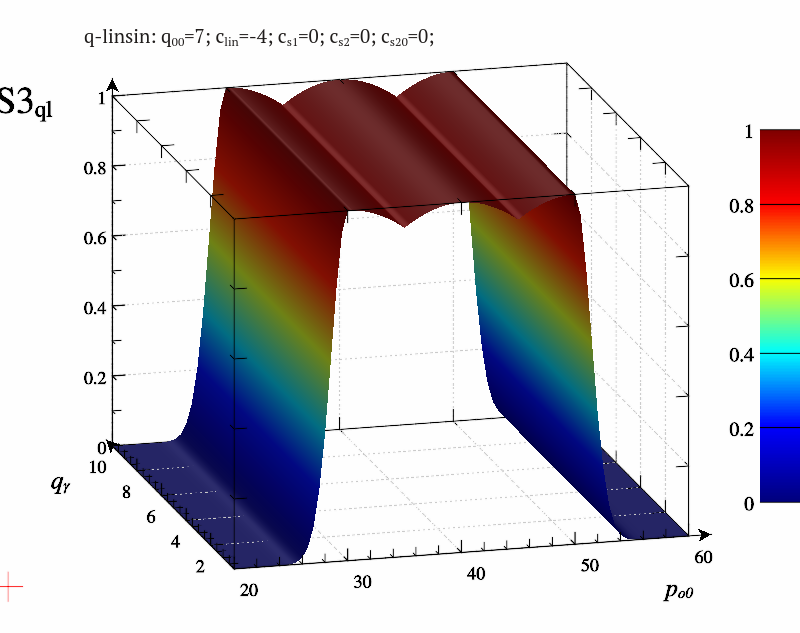
\includegraphics[width=0.32\textwidth]{p/qls_pe-p_po_qg_Sql_lin.png}
    \hfill
    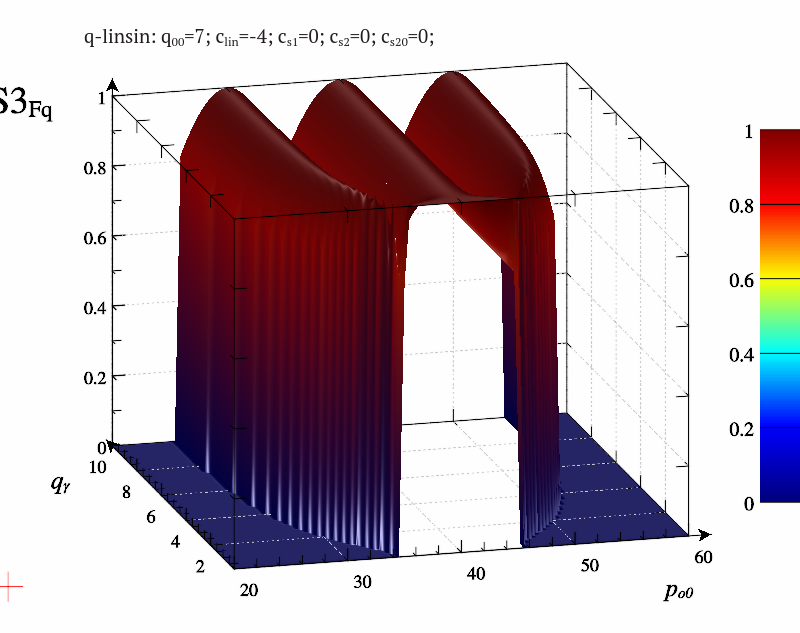
\includegraphics[width=0.32\textwidth]{p/qls_pe-p_po_qg_SFq_lin.png}
    \hfill
    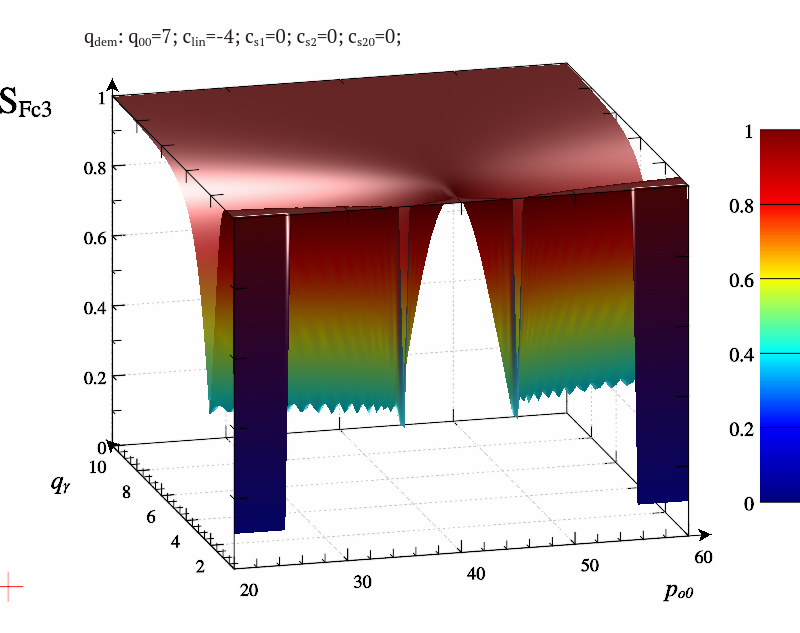
\includegraphics[width=0.32\textwidth]{p/qls_pe-p_po_qg_SFc_lin.png}
  }
  \caption{Зависимости $S(p_o,q_\gamma)$ для методов $p_{eql}$, $p_{eFq}$, $p_{qFc}$ для условий (\ref{atu:eq:q_dem_lin})}
  \label{atu:f:qsl_S_po_qg_lin}
\end{figure}

\begin{figure}[htb!]
  \centerline{
    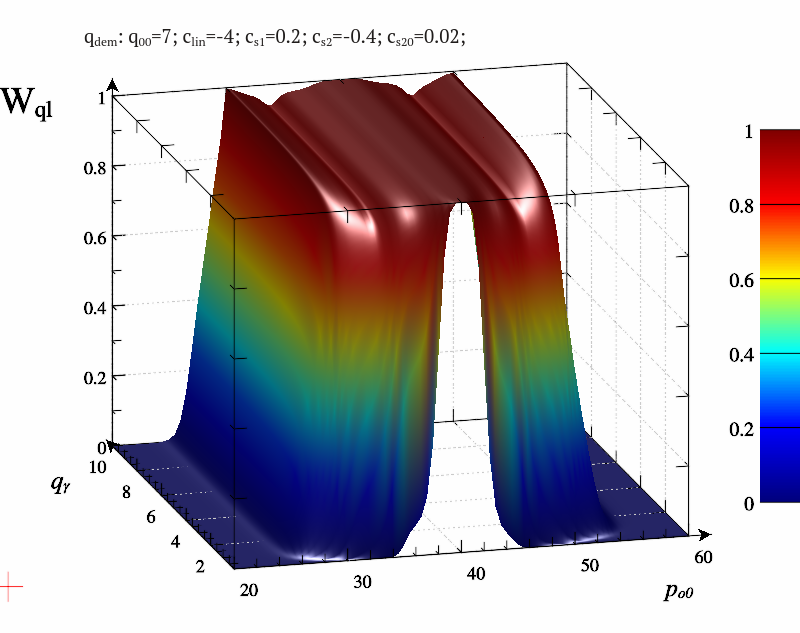
\includegraphics[width=0.32\textwidth]{p/qls_pe-p_po_qg_Wql_all.png}
    \hfill
    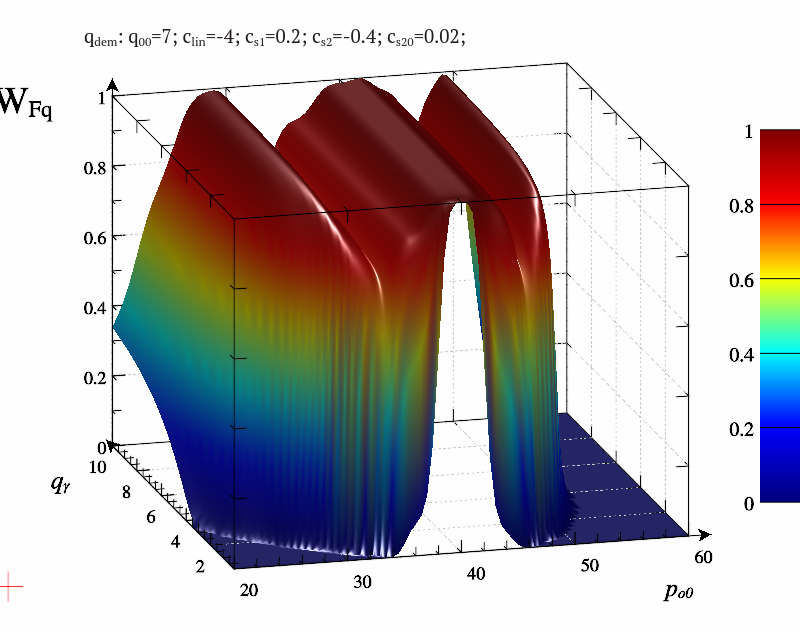
\includegraphics[width=0.32\textwidth]{p/qls_pe-p_po_qg_WFq_all.png}
    \hfill
    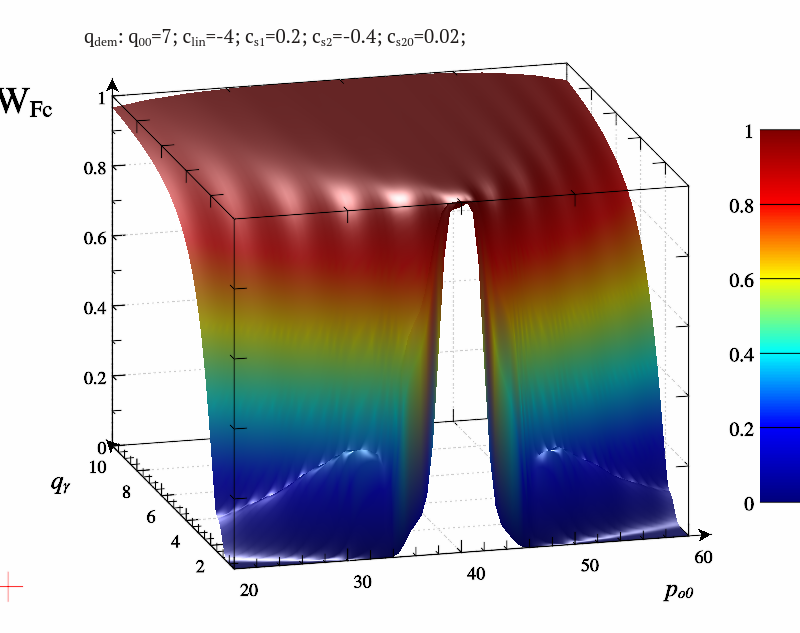
\includegraphics[width=0.32\textwidth]{p/qls_pe-p_po_qg_WFc_all.png}
  }
  \caption{Зависимости $W(p_o,q_\gamma)$ для методов $p_{eql}$, $p_{eFq}$, $p_{qFc}$ для условий (\ref{atu:eq:q_dem_all})}
  \label{atu:f:qsl_W_po_qg_all}
\end{figure}


\begin{figure}[htb!]
  \centerline{
    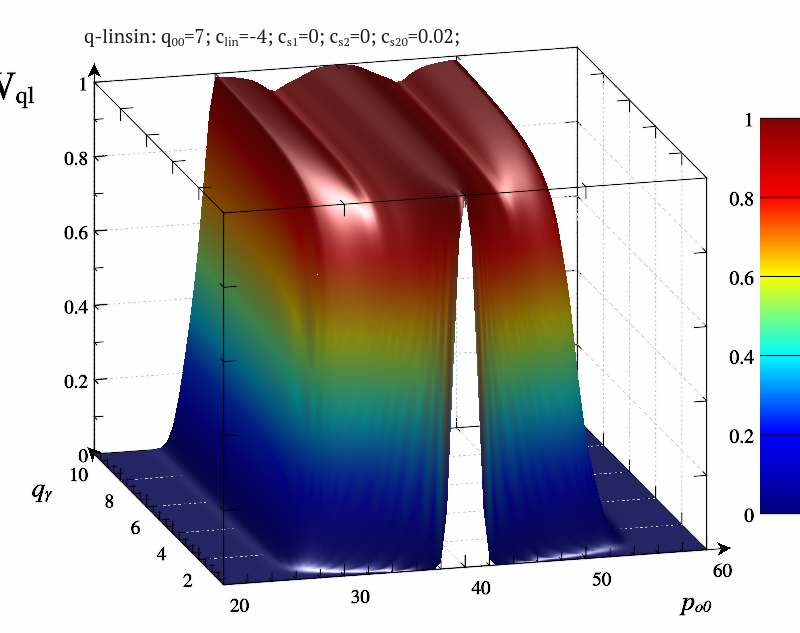
\includegraphics[width=0.32\textwidth]{p/qls_pe-p_po_qg_Wql_s20.png}
    \hfill
    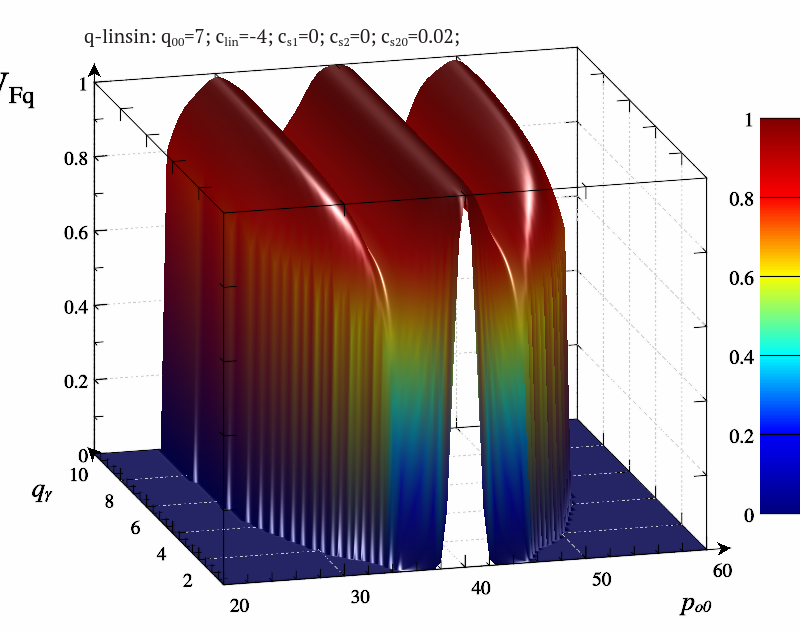
\includegraphics[width=0.32\textwidth]{p/qls_pe-p_po_qg_WFq_s20.png}
    \hfill
    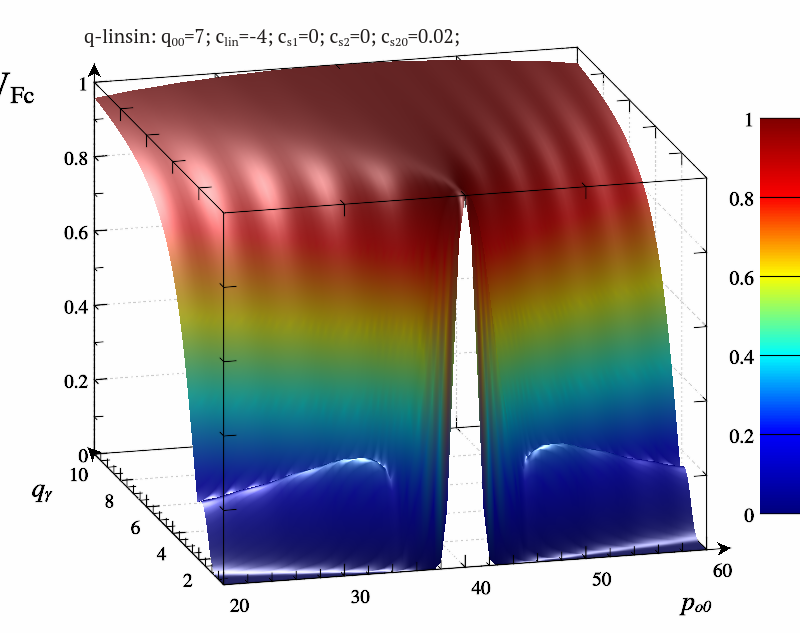
\includegraphics[width=0.32\textwidth]{p/qls_pe-p_po_qg_WFc_s20.png}
  }
  \caption{Зависимости $W(p_o,q_\gamma)$ для методов $p_{eql}$, $p_{eFq}$, $p_{qFc}$ для условий (\ref{atu:eq:q_dem_s20})}
  \label{atu:f:qsl_W_po_qg_s20}
\end{figure}

\begin{figure}[htb!]
  \centerline{
    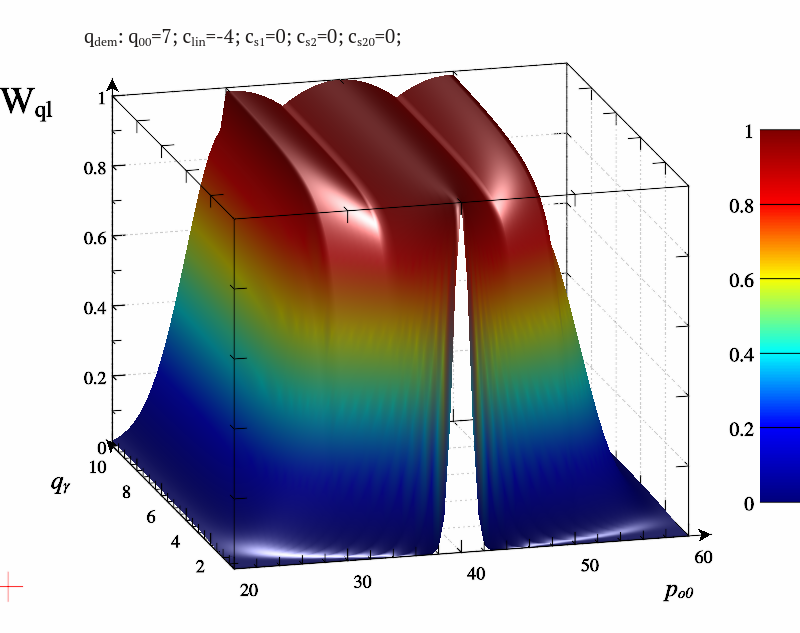
\includegraphics[width=0.32\textwidth]{p/qls_pe-p_po_qg_Wql_lin.png}
    \hfill
    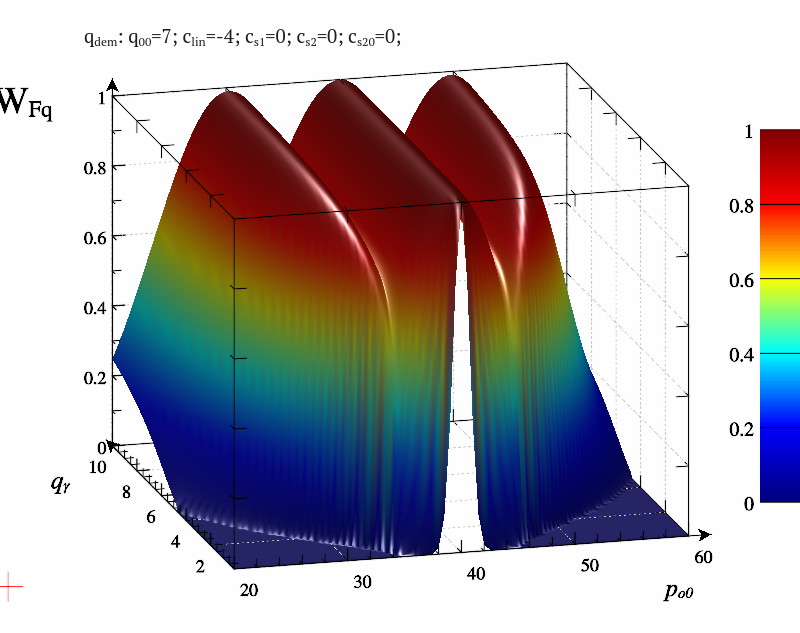
\includegraphics[width=0.32\textwidth]{p/qls_pe-p_po_qg_WFq_lin.png}
    \hfill
    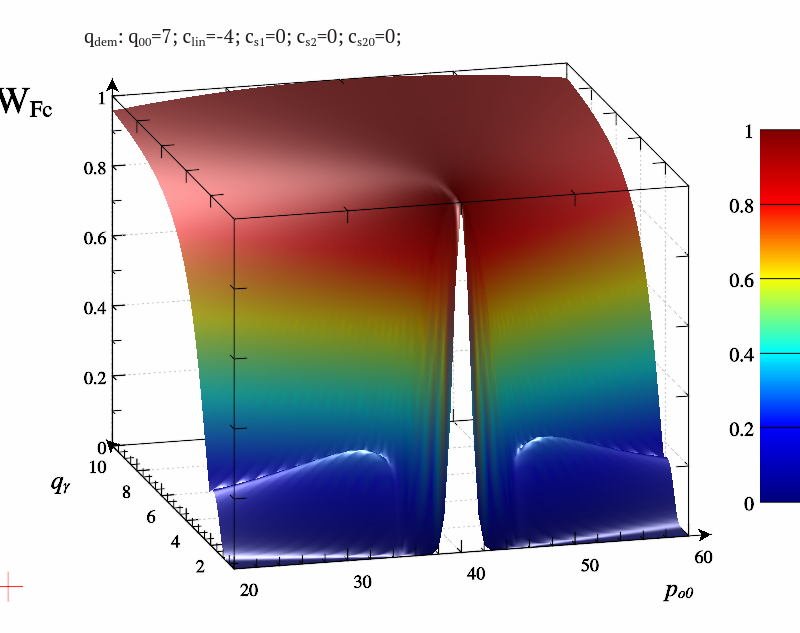
\includegraphics[width=0.32\textwidth]{p/qls_pe-p_po_qg_WFc_lin.png}
  }
  \caption{Зависимости $W(p_o,q_\gamma)$ для методов $p_{eql}$, $p_{eFq}$, $p_{qFc}$ для условий (\ref{atu:eq:q_dem_lin})}
  \label{atu:f:qsl_W_po_qg_lin}
\end{figure}

Во второй серии вычислительных экспериментов
значение параметра объекта
было фиксированным $p_o=39$,
а расстояние между агентами $A$
изменялось от $0.1$ до $20$.
При этом, при $A<1$
точка $p_o$ находилась за пределами интервала $[p_l,p_r]$,
и положение $p_e$ определялось с помощью экстраполяции.

\begin{figure}[htb!]
  \centerline{
    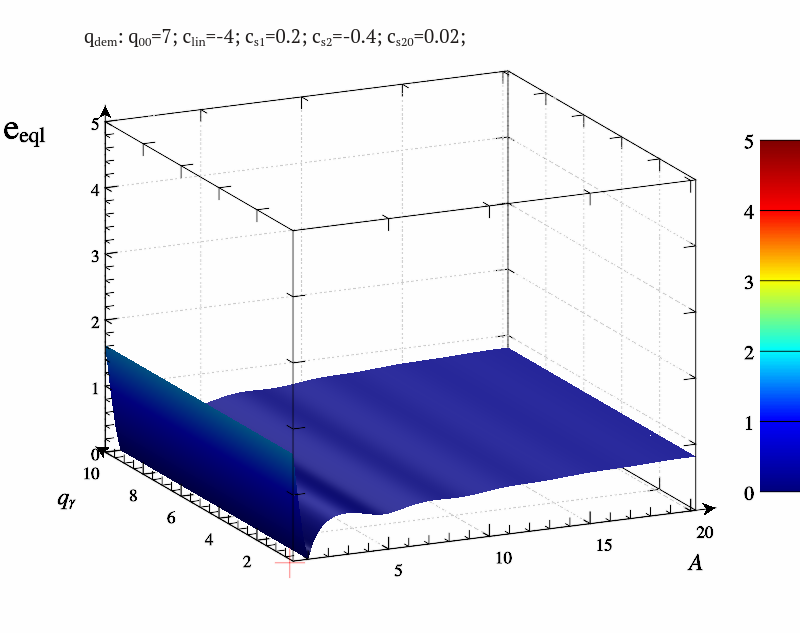
\includegraphics[width=0.32\textwidth]{p/qls_pe-p_A_qg_eql_all.png}
    \hfill
    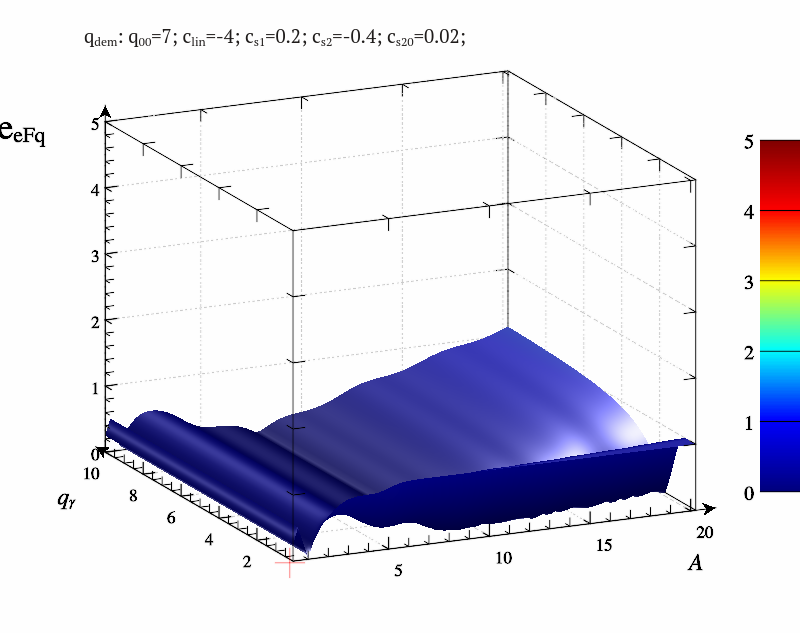
\includegraphics[width=0.32\textwidth]{p/qls_pe-p_A_qg_eFq_all.png}
    \hfill
    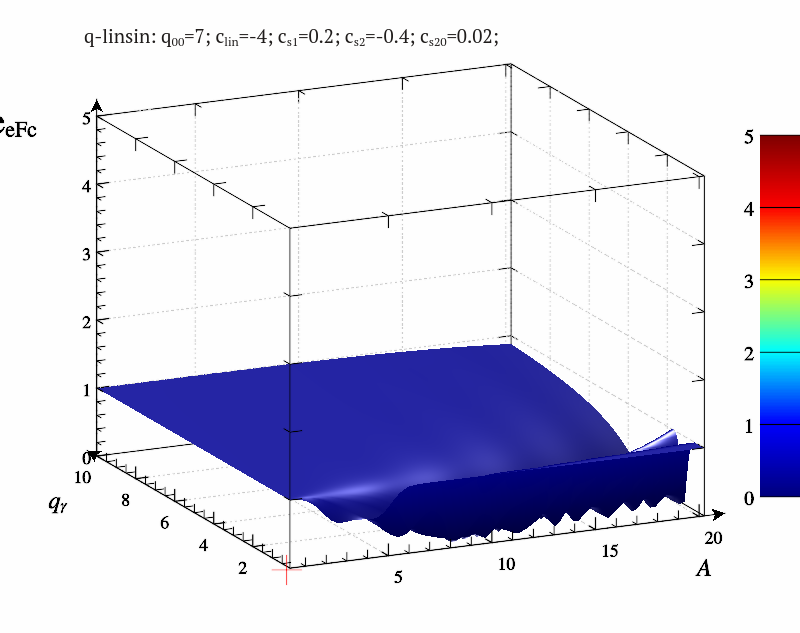
\includegraphics[width=0.32\textwidth]{p/qls_pe-p_A_qg_eFc_all.png}
  }
  \caption{Зависимости $e(A,q_\gamma)$ для методов $p_{eql}$, $p_{eFq}$, $p_{qFc}$ для условий (\ref{atu:eq:q_dem_all})}
  \label{atu:f:qsl_pe_A_qg_all}
\end{figure}


\begin{figure}[htb!]
  \centerline{
    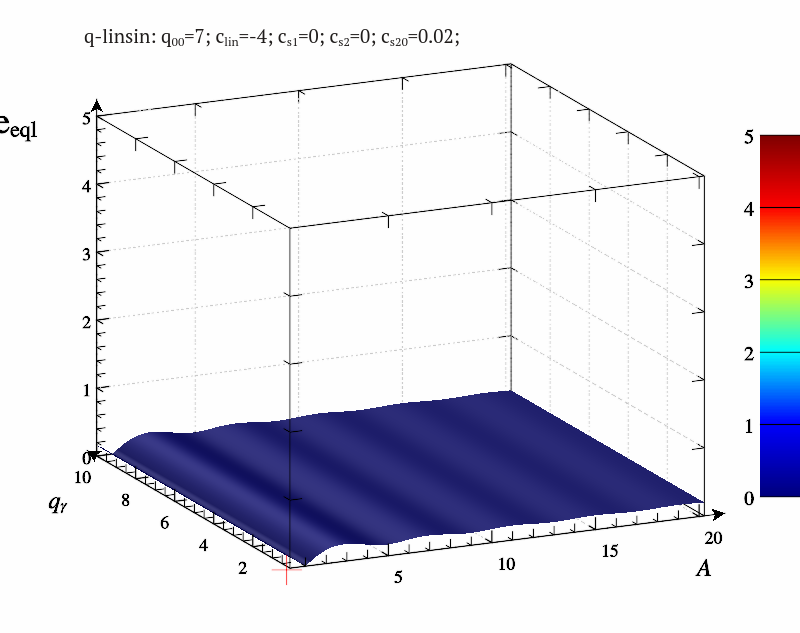
\includegraphics[width=0.32\textwidth]{p/qls_pe-p_A_qg_eql_s20.png}
    \hfill
    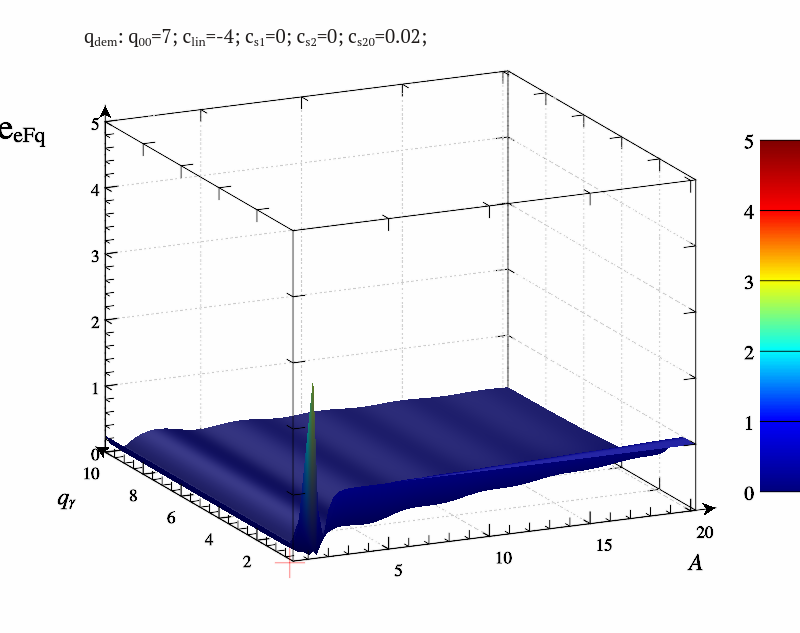
\includegraphics[width=0.32\textwidth]{p/qls_pe-p_A_qg_eFq_s20.png}
    \hfill
    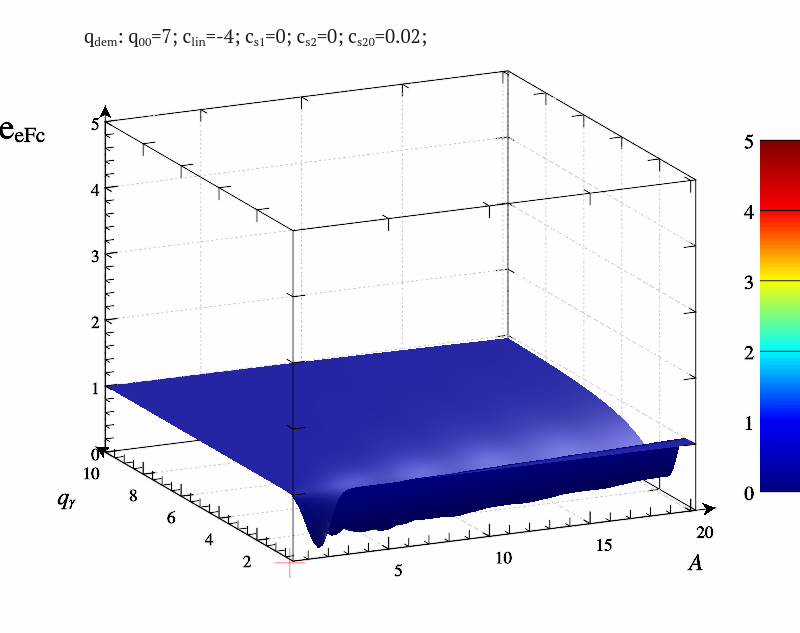
\includegraphics[width=0.32\textwidth]{p/qls_pe-p_A_qg_eFc_s20.png}
  }
  \caption{Зависимости $e(A,q_\gamma)$ для методов $p_{eql}$, $p_{eFq}$, $p_{qFc}$ для условий (\ref{atu:eq:q_dem_s20})}
  \label{atu:f:qsl_pe_A_qg_s20}
\end{figure}

\begin{figure}[htb!]
  \centerline{
    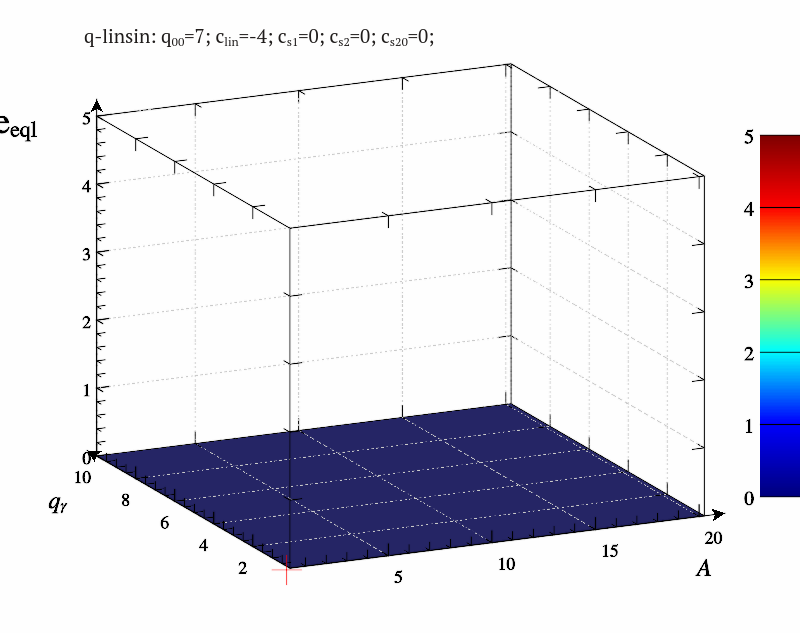
\includegraphics[width=0.32\textwidth]{p/qls_pe-p_A_qg_eql_lin.png}
    \hfill
    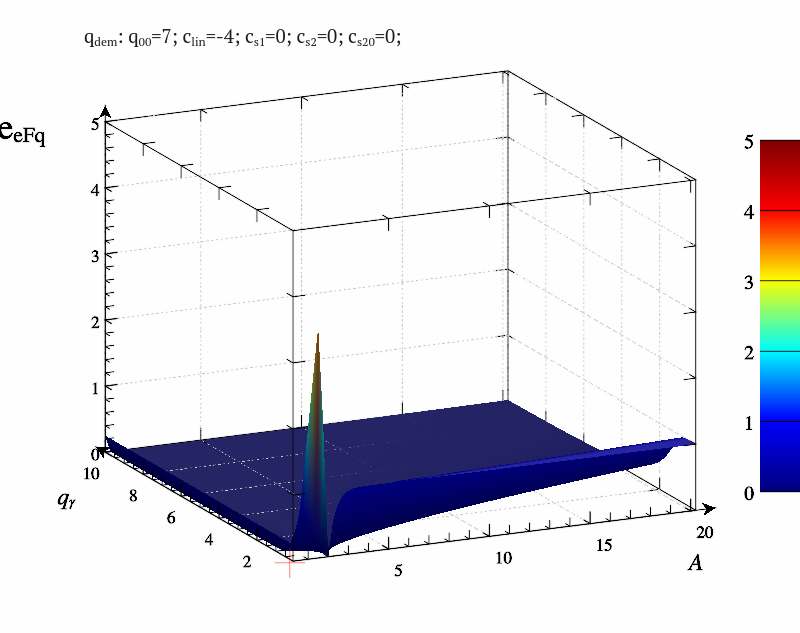
\includegraphics[width=0.32\textwidth]{p/qls_pe-p_A_qg_eFq_lin.png}
    \hfill
    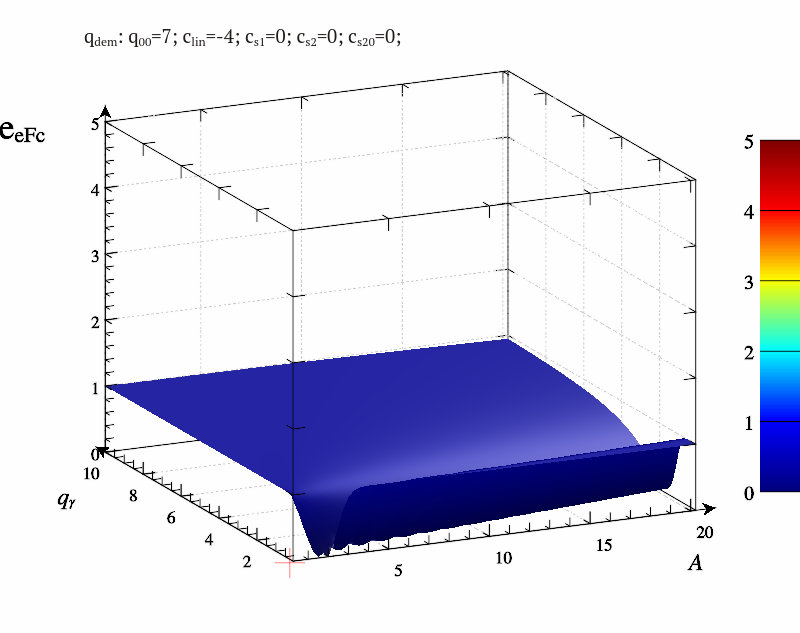
\includegraphics[width=0.32\textwidth]{p/qls_pe-p_A_qg_eFc_lin.png}
  }
  \caption{Зависимости $e(A,q_\gamma)$ для методов $p_{eql}$, $p_{eFq}$, $p_{qFc}$ для условий (\ref{atu:eq:q_dem_lin})}
  \label{atu:f:qsl_pe_A_qg_lin}
\end{figure}



% }}}2

\subsection{Динамика поисковых агентов}  % {{{2

Значение $p_e$, полученное поисковым агентом, может использоваться непосредственно и
мгновенно в качестве значения параметров для управляемых моделей только в том случае,
если объект, и следовательно модели, не проявляют собственной динамики,
то есть являются статическими. Идентификация статических объектов не
является задачей в данной работе.

При моделировании произвольной нелинейной динамической системы,
а особенно хаотических систем, нет возможности строго
определить допустимую динамику изменения параметров
в процессе идентификации. Более того, существуют
даже линейные системы, для которых малые, но специальным
образом подобранные параметрические воздействия
приводят к неограниченному росту значений, отображающих
состояние системы. Одним из самых известных примеров
такого поведения является параметрический резонанс~\Cmt{ref:Sivuhin1}.
Для систем динамического хаоса более известным явлением является
сигнальная синхронизация систем, однако,
возможность аналогичных параметрических влияний достаточно очевидна.

Тем не менее, если исключить достаточно редкие особые случаи,
можно оценить допустимую динамику изменения параметров.
Прежде всего, в процессе синтеза критерия идентификации
одним из этапов является определение корректного значения $\tau_q$.
Чаще всего, данная величина неявно задаёт и допустимую
скорость изменения параметров моделей в процессе идентификации.

При моделировании динамики тела без учёта вращения в механике достаточно
задать все силы, действующие на это тело.
Аналогично, определяя  поисковую динамику агента
требуется определить эквивалент ``сил'',
вызывающих смещение параметров моделей, контролируемых агентом.
При этом задачу определения динамики можно упростить,
разделив ``силы'' на две группы. В первую входят
силы, приводящие к ``движению''. Во вторую входят силы сопротивления,
и вместо рассмотрения самих сил достаточно
определить правила динамики, при этом возможно
использование правил, не имеющих прямого отображения
на реальные физические системы.
Такое разделение позволяет позволяет более простым образом классифицировать
способы задания поисковой динамики.


\subsubsection{Определения сил, используемых при описании динамики поискового агента}  % {{{3

Рассмотрим способы определения основных действующих сил.

$f_e$ --- ``сила притяжения'' к локальной
оценке $p_e$, обеспечивает смещение агента в направлении этой точки,
и, следовательно, увеличению ``плотности'' агентов в окрестностях $p_o$.
Рассмотрим возможные способы определения.

Самым простым,  очевидным, и имеющим прозрачный физический смысл является
следующее определение:
%
\begin{equation}
  f_e(t) = - k_e \left( p_c(t) - p_e(t) \right)  ,
  \label{atu:eq:f_e_lin}
\end{equation}
%
где $k_e$ --- коэффициент пропорциональности, соответствующий
коэффициенту жёсткости условной ``пружины'', деформирующейся
при удалении $p_c$ от $p_e$. Это определение достаточно универсально,
и имеет смысл при реализации многих поисковых тактик. Тем не менее,
это определение не лишено недостатков. Прежде всего,
потенциальная яма, образованная силой вида~(\ref{atu:eq:f_e_lin}),
имеет параболическую форму, и если агент находится на дне этой
ямы, малые внешние силы легко выводят агента из центра данной ямы,
что, в свою очередь, может приводить к снижению точности идентификации.

Вышеупомянутого недостатка лишено следующее определение:
%
\begin{equation}
  f_e(t) = - k_e \sign \left( p_c(t) - p_e(t) \right) ,
  \label{atu:eq:f_e_sign}
\end{equation}
%
образующее треугольную потенциальную яму. При этом,
устранение одного недостатка приводит к появлению
нескольких других. Прежде всего, наличие разрыва
этой функции требует принятия специальных мер по обеспечению
вычислительной устойчивости алгоритмов при
численном моделировании. С другой стороны,
постоянное значение этой функции при отдалении
$p_c$ от $p_e$ может привести к снижению скорости поиска.
В первую очередь этому недостатку будут подвержены
методы идентификации с одним агентом.

Промежуточный способ определения рассматриваемой ``силы''
даёт следующее определение:
%
\begin{equation}
  f_e(t)
  = - k_e \cdot
  \begin{cases}
    1 &  p_c(t) - p_e(t)  > p_\mathrm{sat}
    \\
    \frac{p_c(t)-p_e(t)}{p_\mathrm{sat}} & | p_c(t)-p_e(t)| \le p_\mathrm{sat}
    \\
    -1 &  p_c(t) - p_e(t)  < -p_\mathrm{sat}
  \end{cases},
  \label{atu:eq:f_e_sat}
\end{equation}
%
где  $p_\mathrm{sat}$ --- малая по сравнению с областью поиска величина.
Это определение в какой-то мере объединяет преимущества и недостатки
двух предыдущих.  Нет разрыва в нуле, малые внешние возмущения
приводят к достаточно ограниченным смещениям, но
ограниченность этой зависимости, как и предыдущей,
делает неудобным использование этого определения для систем с одним агентом.

Общим недостатком определения силы $f_e$ по выражениям
(\ref{atu:eq:f_e_lin})--(\ref{atu:eq:f_e_sat})
является то, что сила определяется только по локальным параметрам
в окрестности агента.
Более того, игнорируется даже локальное значение уверенности агента в оценке $p_e$.
Для агентов, находящихся в непосредственной близости к
$p_o$, такое определение силы оправданно. Все остальные агенты
в случае правильного определения направления, будут этой силой прижиматься
к краю своей полосы, если она есть, или же проявлять тенденцию
к сильному скучиванию в противном случае. Более того,
для агентов, находящихся вдали от искомого значения, влияние ошибок измерения
приводит к постоянной смене оценки направления к $p_o$, и как
следствие --- к сильному ``рысканью'' таких агентов.
Следовательно, необходимо ограничение этой силы,
на основании локальных, глобальных, или же и тех и других оценок.
Например:
%
\begin{equation}
  f_e(t) = - k_e S_e(t) \left( p_c(t) - p_e(t) \right) ,
  \label{atu:eq:f_e_lin_S}
\end{equation}
%
\begin{equation}
  f_e(t) = - k_e F_c(t) \left( p_c(t) - p_e(t) \right) ,
  \label{atu:eq:f_e_lin_F}
\end{equation}
%
\begin{equation}
  f_e(t) = - k_e W(t) \left( p_c(t) - p_e(t) \right) ,
  \label{atu:eq:f_e_lin_W}
\end{equation}

\Cmt{примеры}

Наличие только силы $f_e$ приводит к тому, что поведение агентов
будет практически независимым, и для реализации свойств
``ансамбля'' агентов необходимо введение сил,
регламентирующих коллективное поведение.
В первую очередь, следует определить силу $f_n$,
определяющую взаимодействие агента с ближайшими соседями.
В достаточно общем случае эту силу можно определить как
%
\begin{equation}
  f_n( p_r, p_c, p_l ) = f_{nr}(p_r-p_c) + f_{nl}(p_c-p_l).
  \label{atu:eq:f_n_gen}
\end{equation}

В случае линейности и одинаковых определений функций $f_{nr}$ и $f_{nl}$
эта зависимость приобретает вид
%
\begin{equation}
  f_n = k_n ( p_r - 2 p_c + p_l ),
  \label{atu:eq:f_n_lin}
\end{equation}
%
где $k_n$ --- масштабный коэффициент, соответствующий
коэффициенту жёсткости ``пружин'', соединяющих агенты.
При этом следует отметить, что эта функция будет принимать нулевые значения
при любом равномерном распределении агентов, вне зависимости
от расстояния между ними. И, соответственно, будет
противодействовать влиянием, приводящим
к неравномерному распределению. При
этом нет понятия ``естественного расстояния''
между объектами, на котором они находятся в состоянии
устойчивого равновесия при $f_e = 0$.

При определённых соотношениях между $k_e$ и $k_n$
возможна ситуация, когда траектории двух агентов пересекаются.
Для некоторых типов агентов, например, использующих для
оценки $p_e$ \Cmt{TODO: def and ref локальный COG},
это не представляет проблемы. Для большинства других
наличие таких пересечений представляет собой случай,
когда метода определения $p_e$ даёт принципиально
неверные, в том числе неопределённые результаты.
Одним из способов недопущения подобных состояний
является назначение агентам непересекающихся рабочих диапазонов.
Другим --- использование нелинейной функции $f_n$,
обеспечивающей сильное, вплоть до неограниченного отталкивание
агентов при сближении, например:
%
%
\begin{equation}
  f_n = k_n \left( \log\left( \frac{p_r-p_c}{p_{d0}} \right) -  \log\left( \frac{p_c-p_l}{p_{d0}}\right) \right),
  \label{atu:eq:f_n_log}
\end{equation}
%
где
$p_{d0}$ --- ``естественное'' расстояние между агентами, обычно равное начальному расстоянию:
$p_{d0} = \frac{\Delta p}{N-1}$.





Наличие функции $f_n$ обеспечивает определённые аспекты
коллективного поведения агентов, противодействуя неоправданной
скученности агентов. Том не менее, наличие этой функции во многих задачах
недостаточно для построения работоспособной системы идентификации.
В первую очередь, вид этой функции не препятствует равномерному
сжатию или растяжению, противодействие вызывает лишь неравномерность этих процессов.
Более того, ``пилообразная'' зависимость параметра объекта от времени
может приводить к ситуации, когда  значение параметра агента будут
отслеживать последовательно разные агенты, и как следствие,
весь ансамбль агентов будет
последовательно смещаться в одну сторону.
Таким образом, требуется как минимум ещё одна сила,
которая будет препятствовать таким нежелательным эффектам.
В качестве такой силы можно использовать
$f_c$  --- ``силу притяжения'' к начальному значению
параметра ($p_{c}(0)$)
для данной модели. В линейной постановке эта сила определяется как
%
\begin{equation}
  f_c = -k_c (p_c - p_{c}(0)) ,
  \label{atu:eq:f_c}
\end{equation}
%
где $k_c$ --- коэффициент, соответствующий жёсткости ``пружины'',
связывающей агента с его начальным положением, то есть в какой-то
мере ``привязывающей'' его к определённому диапазону
в пространстве параметров.

Наличие сил $f_n$ и $f_c$ не даёт всем моделям принять одно
и то же значение параметра вблизи экстремума, и, следовательно,
прекратить процесс поиска. Это также позволяет быстро переключиться
на другую модель в случае быстрого изменения параметра объекта.

Результаты моделирования показали, что в большинстве случаев
имеет смысл введение дополнительных сил ``барьерного'' вида,
для исключения пересечения траекторий поисковых агентов,
или же их ухода из рабочего диапазона.

Системы идентификации с одним агентом не требуют описания
динамики коллективного поведения, и для
них силы $f_n$ и $f_c$ разумно считать нулевыми.
Тем не менее, в этом случае постановка задачи может потребовать
ограничения значений параметра модели. Этого можно достичь
как введением дополнительных функций ``барьерного''
вида на границе, так и алгоритмическими ограничениями.

% TODO: searching force

С учетом вышеизложенного, определим
сумму всех ``сил'', действующих на поисковый агент:
\begin{equation}
  f_t = f_c + f_n + f_e .
  \label{atu:eq:f_t}
\end{equation}


% }}}3



\subsubsection{Способы определения поисковой динамики агента при заданной силе}  % {{{3

\paragraph{Метод ``тяжёлого шарика''}

В этом случае поисковая динамка задаётся следующим образом~\Cmt{ref}:
%
\begin{equation}
  m \ddot{p}_c + \nu \dot{p}_c = f_t(t),
  \label{atu:eq:heavy_ball}
\end{equation}
%
где $m$ --- эквивалент массы шарика,
$\nu$ --- коэффициент условной вязкости.
Применение этого подхода оправданно,
в первую очередь, при использовании системы идентификации с одним поисковым агентом.
В этом случае ослабляются требования на монотонность зависимости $q(p)$,
или же одноэкстремальности $F(p)$.
К недостаткам данного подхода следует отнести
большие вычислительные затраты,
и повышенные требования к устойчивости поиска.


\paragraph{Метод ``вязкой динамики''}

В приближении динамики тела в вязкой жидкости,
когда влияние инерции пренебрежимо мало по сравнению  с вязкостью,
изменения параметров моделей (поисковых агентов) задаётся следующим образом:
%
\begin{equation}
  \od{p_c}{t} = v_f f_t(t),
  \label{atu:eq:v_f}
\end{equation}
%
\noindent
где $f_t$ --- сумма всех действующих ``сил'', $v_f = 1/\nu$ --- коэффициент
пропорциональности. Данный подход,
по сравнению с предыдущим,
требует меньших вычислительных затрат,
и проявляет большую устойчивость. Более слабые поисковые способности
компенсируются применением множества агентов. Поэтому, в дальнейшем
изложении для многомодельных систем будет применяются именно этот подход.

\paragraph{Специальные подходы}

Существуют методы адаптивно-поисковой идентификации,
определяющие свои правила описания поисковой динамики.
При этом, могут не вводится понятия $p_e$, $f_t$  и другие.
Тем не менее, в целом, эти специальные способы определения динамики
можно свести к используемой терминологии.

Так, например, оригинальный адаптивно-поисковый метод~\Cmt{ref}
использует поисковые колебания и для определения скорости смещения,
и для реализации смещения как такового. При этом,
после усреднения на интервале поискового периода,
динамика поиска может быть описана выражением~(\ref{atu:eq:v_f}).

Метод с двумя моделями и двумя УГПК~\Cmt{ref}
также задаёт поисковую динамику
специальным образом. В отличие от предыдущего случая,
для определения скорости смещения параметров используется пара
моделей, и смещение реализуется за счёт разности срабатывания двух УГПК.
Тем не менее, и это случае, после усреднения, динамика
может быть описана выражением~(\ref{atu:eq:v_f}).



% }}}3


% }}}2






% }}}1

\section{Методы, параметры и алгоритмы работы поисковых координаторов}  % {{{1

\subsection{Методы определения значения идентифицируемого параметра координатором поиска} % {{{2


Рассмотрим набор подходов к определению поисковым координатором
точки максимума функции качества, а следовательно --- значения идентифицируемого параметра \cite{atu_st99,atu_jacs2015}.

В качестве первого приближения можно просто в качестве $p_\mathrm{id}$
использовать значение $p_c$ той модели, для которой функция качества максимальна:
%
\begin{equation}
  p_{bm}
  =
  p_{c,i};
  \quad
  i : F_i = \max{F_j}, \, j=0 \ldots N-1 .
  \label{atu:eq:p_b}
\end{equation}

Единственным достоинством данного метода является простота реализации.
При этом, никак не используются аппроксимирующие способности агентов.
Более того, зависимость $p_{bm}(t)$ подвержена
скачкообразным изменением в момент переключения
с одной модели на другую.

Следует отметить, что для методов, использующих
одну модель это практически единственный метод определения $p_\mathrm{id}(t)$.


Следующий метод --- реализация
метода COG (Center of gravity, Такаги-Сугено) \cite{atu_asau25,atu_csit2015,atu_asau16},
используемого при дефаззификации систем нечёткой логики:
%
\begin{equation}
  p_{ge}
  =
  \frac{\sum\limits_{i=0}^{N-1} F_{i} p_{i}}
       {\sum\limits_{i=0}^{N-1} F_{i} }
  .
  \label{atu:eq:p_ge}
\end{equation}

Этот метод можно модифицировать, используя аппроксимирующие свойства самих агентов.
Для этого в качестве значения параметра в формуле (\ref{atu:eq:p_ge})
вместо текущего значения параметра $p_c$ агента следует использовать
аппроксимированное значение $p_e$, обозначив его для
модели номер $i$ как $p_{e,i}$. Так как этому значению
параметра не соответствует ни одной модели, то и значение функции
качества для этой точки неизвестно. Предлагается вместо
значения $F$ в этом случае использовать произведение
$F_i \cdot S_i$. Тогда обозначим
%
\begin{equation}
  p_{xe}
  =
  \frac{\sum\limits_{i=0}^{N-1} F_{i} S_i p_{e,i}}
       {\sum\limits_{i=0}^{N-1} F_{i} S_i }
  .
  \label{atu:eq:p_xe}
\end{equation}

Использование в подобных выражениях только $S_i$ без $F_i$
практического смысла не имеет,
так как $S-i$ --- локальное свойство агента, и этом случае агенты,
находящиеся вдали от искомой точки, но ``достаточно уверенно'' определившие $p_e$
на основании локальных возмущений, будут учитываться наравне с теми
агентами, которые в самом деле близки к искомому значению $p$.

Следующий подход призван уменьшить зависимость первого
от влияния локальных экстремумов и границ. В этом
случае определяется модель $M_{i_{m}}$ с максимальным значением
$F$, а в оценке используется только ближайшая окрестность этой модели:
%
\begin{equation}
  p_{le}
  =
  \frac{ F_{i-1} p_{i-1} + F_{i} p_{i} + F_{i+1} p_{i+1} }
       { F_{i-1}         + F_{i}       + F_{i+1}         }
  ;
  \quad
  i : F_i = \max{F_j}, \, j=0 \ldots N-1 .
  \label{atu:eq:p_le}
\end{equation}
%
или, с учётом введённых локальных обозначений при $i=c$:
%
\begin{equation}
  p_{le}
  =
  \frac{ F_{l} p_{l} + F_{c} p_{c} + F_{r} p_{r} }
       { F_{l}       + F_{c}       + F_{r}       }
  .
  \label{atu:eq:p_lel}
\end{equation}

Ошибки идентификации в пространстве параметров
для рассмотренных трёх подходов обозначим соответственно:
%
\begin{equation}
  e_{ge} = p_{ge} - p_o,
  \quad
  e_{le} = p_{le} - p_o,
  \quad
  e_{ee} = p_{ee} - p_o,
  \quad
  e_{xe} = p_{xe} - p_o.
  \label{atu:eq:e_xx}
\end{equation}




% }}}2


% }}}1


\section{Классификация и обозначения систем идентификации}  % {{{1
\label{atu:id_classification}

В данной работе рассматривается набор методов идентификации нелинейных динамических
систем. При этом, большинство из них имеют общие свойства, и система идентификации в  целом
состоит из ``набора'' модулей и алгоритмов, комбинация которых
позволяют выбрать конкретный метод, подходящий для данной задачи.
Следовательно, возникает вопрос корректного и непротиворечивого обозначения
используемого метода. Ввиду значительного количества методов, полученных
путём комбинации их элементов, не имеет смысла давать каждому
отдельное названия. Возникает потребность в унификации обозначений
методов, и соответственно, введения определённой классификации.

Предлагается к использованию следующая система обозначений:

\begin{enumerate}

  \item  Первый символ определяет, какая величина ($q$ или $F$) используется
    каждым агентом для определения $p_e$. Соответственно, первый символ
    будет ``q'' или ``F''.
    Для обозначения методов, для которых в качестве критерия используется
    непосредственно выходы моделей и объектов, использует символ ``x''.
    При необходимости, при появлении новых подходов,
    могут быть назначены дополнительные символы.

  \item
    Второй символ задаёт способ определения идентифицируемого параметра по всему ансамблю:
    \begin{description}

      \item[b]  --- ``best'' --- выбирается лучший агент без дальнейшей обработки;

      \item[g]  --- ``global COG'' --- метод ``Center of Gravity'' по всему ансамблю~(\ref{atu:eq:p_ge});

      \item[l] --- ``local COG'' ---   метод ``Center of Gravity'' по окрестности лучшего агента~(\ref{atu:eq:p_le});

      \item[e] --- квадратическая интерполяция по $F$ в окрестности лучшего агента~(\ref{atu:eq:p_eFq});

      \item[x] --- ``extremum COG'' --- вариант ``Center of Gravity'' по всему ансамблю, при этом
        от каждого агента используются величины $p_e$ и $FS_e$.

    \end{description}

    В случае, если вместо ансамбля используется 1--2 агента, то для определённости будет
    использован символ ``b''

  \item
    Третий символ обозначает выбранную зависимость для величины $f_e$ (или аналогичной величины, если $f_e$ напрямую не используется):
    \begin{description}

      \item[c]  --- ``const'' --- величина $f_e$ не участвует в описании
        динамики поискового агента;

      \item[l] --- ``linear'' ---  величина $f_e$ линейно зависит
        от $p_e$~(\ref{atu:eq:f_e_lin});

      \item[s] --- ``sign'' --- используется зависимость вида~(\ref{atu:eq:f_e_sign});

      \item[u] --- ``saturate'' ---  используется зависимость вида~(\ref{atu:eq:f_e_sat});

    \end{description}


  \item
    Четвёртый символ указывает, каким образом величина $f_t$ (или её эквивалент) влияет на динамику агента:
    \begin{description}

      \item[z]  --- ``zero'' --- агент неподвижен;

      \item[v] --- ``viscous'' ---  используется модель вязкого трения~(\ref{atu:eq:v_f});

      \item[b] --- ``ball'' --- используется подход ``тяжёлого шарика''~(\ref{atu:eq:heavy_ball});

      \item[s] --- ``special'' --- особый вид, задаётся методом непосредственно.

    \end{description}

  \item
    Пятый символ позволяет указать, какое дополнительное поисковое движение
    реализует агент
    \begin{description}

      \item[n]  --- ``none'' --- дополнительное поисковое движение не используется,
        при этом, если не возникает неоднозначности в классификации, данный символ можно упустить;

      \item[t] --- ``triangle'' ---  используется пилообразное поисковое движение, например, реализуемое
        с помощью УГПК; \Cmt{ref};

      \item[d] --- ``dual'' --- используется поисковое движение, реализуемое, например, парой УГПК;

      \item[s] --- ``sin'' ---  используется гармоническое поисковое движение, применяемое, например, методом синхронного детектора;

      \item[r] --- ``random'' ---  используется случайное поисковое движение (различные варинты случайного поиска).

    \end{description}

  \item
    Следующая группа символов указывает количество активных агентов.
    В одномерном случае это или просто число, или символ ``N'', если
    конкретное количество несущественно. В двумерном случае
    используются варианты ``NxM'' для сеточного расположения агентов,
    и ``NpM'  --- для конфигурации ``крест''. В случае большей размерности
    пространства параметров можно использовать аналогичные обозначения,
    но, при необходимости, с дополнительными индексами, например:
    ``10x10p5'', ``$\mathrm{N_1 p N_2 x N_3 p N_4}$''.

  \item
    Следующий символ, записанный после символа ``.'' указывает количество агентов в
    в поисковой группе, например: ``2'' --- поисковая пара, ``3'' --- триплет.
    При применении методов, использующих только один поисковый агент,
    этот элемент классификации указывает количество моделей, управляемых этим агентом.

  \item Восьмой символ, указываемый при необходимости, описывает
    поведение дополнительных моделей, находящихся на границе:
    \begin{description}

      \item[z]  --- ``zero'' --- реальная модель не используется, функция качества $F$ для неё считается нулевой;

      \item[r] --- ``real'' ---  используется реальная модель, но без возможности её смещения;

      \item[а] --- ``approximate'' --- значение критерия и функции качества каким-то образом аппроксимируются;

    \end{description}

\end{enumerate}

При необходимости, в конец данного обозначения, через точку, добавляется обозначение используемого критерия.
Дополнительное компоненты добавляются в конец после двоеточия. Для обозначения подмножеств методов
вместо обозначения элемента используется символ ``A'' --- ``any''.


Примеры обозначений:

``Fglv5.3z.$q_{x^2}$'' --- Метод, использующий 5 подвижных (3 триплета) и 2 ``fake'' модели,
``global COG'' для результирующего значения параметра
для оценивания величины $p_e$ используется функция качества,
зависимость $f_e$ от $p_e$ --- линейная, ``вязкая'' динамика, критерий ``$q_{x^2}$''.


``qAuv7.3r.$q_{dx}$'' --- Методы, использующий 7 подвижных (5 триплетов) и 2 ``real'' модели на границах,
для оценивания величины $p_e$ используется значение критерия,
зависимость $f_e$ от $p_e$ --- с насыщением, ``вязкая'' динамика, критерий ``$q_{dx}$'',
используются все доступные методы для определения  результирующего значения параметра.

``xblst1'' --- Оригинальный адаптивно-поисковый метод.

``xblvd1.2'' --- Адаптивно-поисковый метод с двумя моделями и двумя УГПК с общим сбросом
 и непосредственным использованием выходов объекта и моделей.

``Fblvd1.2.$q_{x^2}$'' --- Адаптивно-поисковый метод с двумя моделями и двумя УГПК с общим сбросом,
 использующий функцию качества применительно к критерию $q_{x^2}$.

``Fgcz7x7.1'' --- Сетка из 49 ($7 \times 7$) неподвижных моделей,
``global COG'' для результирующего значения параметра,
без указания конкретного критерия.

% }}}1


% ----------------------------------------- ERR -------------------------
\section{Качество идентификации}  % {{{1

Среди множества способов оценивания качества идентификации
можно выделить две группы.
К первой группе относятся те, которые производят оценивание
только на основе критерия идентификации, или,
что в какой-то мере эквивалентно, по функции качества идентификации.
В реальных задачах, когда нет возможности определить реальные значения
параметров объекта, это практически единственный вариант.
При этом подразумевается, что как критерий идентификации, так и
функция качества выбраны корректно.

В процессе синтеза новых критериев и методов идентификации
такой подход, с одной стороны, слишком строг,
с другой --- не даёт проверить корректность полученного результата,
так как в этом случае ни близость критериев модели и объекта,
ни, тем более, близкое к единице значение функции качества не
обозначает работоспособность системы идентификации.
Следовательно, при анализе работоспособности,
которые проводятся как на модельных задачах,
так и на реальных физических объектах в контролируемых
условиях, необходимо использовать методы из второй группы,
основанные на сравнении собственно параметров модели и объекта,
то есть на оценивании параметрической
ошибки идентификации $e(t)=p_o(t)-p_\mathrm{id}(t)$.

В работах [cipkin,myPphd,xxx] были предложены информационные методы
оценивания качества идентификации.
Они отличаются универсальностью, и отображают
успешность решения одной из основных задач
идентификации --- получения информации то объектах.
Однако, для построения информационных оценок
требуется значительно больше ресурсов, чем
для проведения собственно идентификации. В некоторых случаях,
например, при получении данных с реального оборудования,
это может быть просто невозможно.



При таких условиях, качество идентификации для процесса
в целом задаётся мерой:
%
\[
  \overline{e} = \mu( p_o(t), p_\mathrm{id}(t) ),
  \quad
  t \in [0;T].
\]

Конкретный вид меры определяется задачей.
Если в конкретной постановке важно знать максимальное
отклонение идентифицируемого параметра модели от объекта,
то имеет смысл выбрать меру $C[0;T]$~\cite{kolmogorov_fun_ana} или же
$R_{\infty}^n$ для дискретного представления:
%
\begin{equation}
  \overline{e_c}(p_o(t),p_\mathrm{id}(t))
  =
  \max \big| p_o(t)-p_\mathrm{id}(t) \big|,
  \quad
  t \in [0;T].
  \label{atu:eq:e_c}
\end{equation}

Более распространённым является случай,
когда интерес представляет не максимальное значение $|e(t)|$,
а какой-то вариант усреднения этой величины, например
%
\begin{equation}
  \overline{e_2}(p_o(t),p_\mathrm{id}(t))
  =
  \sqrt{ \frac{1}{T} \int\limits_{0}^{T} \big( p_o(t)-p_\mathrm{id}(t) \big)^2 \, \mathrm{d}t },
  \label{atu:eq:e_2}
\end{equation}
%
или
\begin{equation}
  \overline{e_1}(p_o(t),p_\mathrm{id}(t))
  =
  \frac{1}{T} \int\limits_{0}^{T} \big| p_o(t)-p_\mathrm{id}(t) \big| \, \mathrm{d}t .
  \label{atu:eq:e_1}
\end{equation}
%
Этот подход особенно оправдан в тех случаях, когда
значение параметра объекта претерпевает резкие изменения.
При этом, никакая система идентификации не будет успевать за такими
изменениями, особенно с учётом времени, необходимого для
оценивания критерия. Следовательно, если оценивать в таких условиях
качество идентификации, используя \ref{atu:eq:e_c},
то в качестве результата получим всего лишь величину
скачков параметра, а не какие-либо характеристики процесса идентификации.

В тех, достаточно редких случаях, когда из априорной
информации о системе известно, что $p_o(t) = \mathrm{const}$,
имеет смысл в выражениях~(\ref{atu:eq:e_c})--~(\ref{atu:eq:e_1})
ограничить диапазоны для времени, например $[T-\tau_p,T]$,
где $\tau_p$ --- время, достаточное для измерения
критерия идентификации с требуемой точностью.
Это позволит избежать влияния переходных процессов
идентификации на интегральную оценку ошибки.
В остальных случаях, представляет интерес именно реакция
на изменения параметра, поэтому в данной работе преимущественно будет
использоваться выражение~(\ref{atu:eq:e_2}).




Само значение как ошибки идентификации, так и соответствующей меры --- величина размерная,
и в таком виде не пригодно для
независимого от конкретной ситуации оценивания качества работы метода.
Рассмотрим возможные величины, дающие возможность привести ошибку идентификации
к безразмерному виду.

В первую очередь, предположим, что вообще не проводим никакой идентификации,
а в качестве значения параметра используем или геометрический центр $p_{00}$ множества $\mathcal{P}$,
или, если это по какой-либо причине известно, точку с максимальным значением плотности вероятности.
Тогда обозначим
%
\begin{equation}
  \overline{e}_{00}
  =
  \overline{e}(p_o(t),p_{00})
  \label{atu:eq:e_00}
\end{equation}

Относительные ошибки для соответствующих абсолютных~(\ref{atu:eq:e_xx})
тогда будут определены следующим образом:
%
\begin{equation}
  \overline{e}_{rge} = \frac{\overline{e}_{ge}}{\overline{e}_{00}}, \;
  \overline{e}_{rle} = \frac{\overline{e}_{le}}{\overline{e}_{00}}, \;
  \overline{e}_{xee} = \frac{\overline{e}_{xe}}{\overline{e}_{00}}, \;
  \overline{e}_{ree} = \frac{\overline{e}_{ee}}{\overline{e}_{00}}.
  \label{atu:eq:e_rxx}
\end{equation}

Близость этих величин к единице свидетельствует о том, что
данный метод идентификации в рассматриваемых условиях бесполезен.
Более того, при серьёзных нарушениях в процессе поиска,
например при потере устойчивости, эти величины могут и превосходить единицу.

Несмотря на очевидную пользу, такой способ приведения к безразмерному виду ошибок
имеет ряд недостатков. Во-первых,
не учитывается возможная мультиагентная структура системы идентификации,
для которой оценка ~(\ref{atu:eq:e_00}) будет слишком грубой.
С другой стороны,
не учитываются свойства
самой системы. Например, возможна такая ситуация, когда параметр
объекта изменяется настолько быстро (по отношению к времени оценивания критерия),
что любой метод идентификации будет бесполезен.

Для оценивания качества работы системы идентификации с счётом
множества моделей, можно воспользоваться несколькими приёмами.
Первый --- пусть все агенты неподвижны, а в качестве $p_\mathrm{id}(t)$
используется $p_c$ той модели, функция качества для которой
максимальна. Обозначим полученное таким образом значение
параметра как $p_{bm}(t)$ (``best model''),
соответствующую ему усреднённую ошибку как $\overline{e}_{bm}$.
При этом безразмерные величины обозначим как
$\overline{e}_{gebm}$, $\overline{e}_{lebm}$,  \ldots.
Близость этих величин к единице, при одновременной малости
$\overline{e}_{r*}$, свидетельствует о том, что передвижения
агентов практически бесполезны, и работоспособность системы идентификации достигается
практически только за счёт переключения между агентами.
Одной из причин такого поведения, при условии отсутствия ошибок
в настройке системы, может быть высокая чувствительность
объекта к \textit{динамике} изменения параметра, например
при параметрическом резонансе. \Cmt{динамика $p_o(t)$}.

Аналогичный способ, но с учётом возможностей агентов
к аппроксимации --- $p_\mathrm{id}(t)$ определятся
как $p_e(t)$ для лучшего агента.
Соответствующую величину для обезразмеривания обозначим как
$\overline{e}_{ba}$ (``best approximation'').
Отношение $\overline{e}_{bm} / \overline{e}_{ba}$
характеризует аппроксимирующую способность агентов.


\Cmt{ TODO: implement!}
Преодолеть второй недостаток представляется не настолько тривиальной задачей.


Для оценивания возможностей системы идентификации
отслеживать как гладкие, так и скачкообразное изменения параметров,
предлагается для каждой тестовой системы, если это возможно,
проводить моделирование процессов идентификации при условии, что
изменение значения параметра объекта описывается одним из
следующих выражений:
%
\begin{equation}
  p_o(t) = p_0 +  U_{p} \sign \sin( \omega_{p} t ),
  \label{atu:eq:po_t_sign}
\end{equation}
%
%
\begin{equation}
  p_o(t) = p_0 +  U_{p} \sin( \omega_{p} t ).
  \label{atu:eq:po_t_sin}
\end{equation}


При этом, использование зависимости вида~(\ref{atu:eq:po_t_sign})
позволяет определить как реакцию системы на скачкообразные
изменения параметра, так и проверить устойчивость процесса поиска.
Использование зависимости~(\ref{atu:eq:po_t_sin}) позволяет проверить
качество ``сопровождения'' системой идентификации плавно изменяющегося параметра,
и, как правило, в этом случае ошибка идентификации должна быть меньше.








% }}}1

\section{Разновсякое --- переместить}  % {{{1

\paragraph{Требования к поисковым алгоритмам и методам оценивания $p_o$}.

При линейной зависимости $q(p)$ и отсутствии ошибок измерения
ошибка оценивания ``своей'' точки $p_e$ должна быть пренебрежимо малой.

При этих же условиях глобальные оценки $p_o$ также должны
характеризоваться достаточно малыми ошибками.

Сближение и удаление поисковых агентов в пределах назначенных
диапазонов не должно приводить к существенному изменению величины
идентифицируемого значения.

\paragraph{TODO3}.

Определить масштабы времени, параметра, критерия на основании точности измерений,
динамики объекта и системы.

Глобальные и локальные параметры поиска.

Учесть, что $q_o(p) \ne q_m(p)$ --- на самом деле просто игнорируем, или же учитываем при определении допустимой точности.

Корректно определить динамические параметры агента: $v_f$, $k_e$ \ldots
с учётом различных тактик.

Равновесные конфигурации поисковых агентов.

Потенциал a-la Van-dev-Vaald для межагентного взаимодействия.

Почему в тесте linlin(Colp) ee=xe?

Сложность и неоднородность $q(p)$

Определить устойчивость как одного агента, так и системы идентификации в целом.






% }}}1

\section{Выводы по разделу 3}  % {{{1

Выводы.

% }}}1

% \subsection{Время и история}  % {{{2
%
% Способы учёта истории системы и динамических характеристик.
%
% Явное представление истории --- каждый агент имеет способ хранения и использования
% информации о предыдущих значениях параметра и критерия.
%
% Неявное представление истории --- тот факт, что в данный момент времени известно
% текущее значение параметра и критерия, с учетом известных значений
% параметров поиска самого агента, может неявно дать ограниченную информацию
% о предыдущем состоянии.
%
% Стабильные/мобильные модели.
%
% История: локальная + глобальная


% }}}2

% vim: fdm=marker foldlevelstart=2 fdc=4 ft=tex
% \section{Адаптация параметров и состояния элементов поисковых систем}  % {{{1
%
% Какие параметры системы идентификации можно адаптировать
% и на каком уровне.
%
% \Cmt{Когда имеет смысл играть с чувствительностью.}
%
% \Cmt{Как близко имеет смысл подводить модели к экстремуму? --- это не совсем здесь, это есть и свойствах агента}
%
% % }}}1
